\chapter{Konzeption}
\label{cha:konzept}
In diesem Kapitel wird ein Konzept vorgestellt, das alle in dieser Arbeit besprochenen Mechanismen und Anforderungen herkömmlicher Kommunikationsprotokolle umfasst. Die Anforderungen werden zunächst in drei Hauptkategorien eingeteilt:
\begin{itemize}
\item Anforderungen, die inhärent in der Ausführung von Self-Assembly durch DNA-Tiles sind,
\item Anforderungen, die speziell für die Kommunikation mit DNA-Tile-basierten Systemen definiert werden müssen,
\item Anforderungen, die auf der Nanoebene nicht umgesetzt werden sollten, da sie sich besser für eine Implementierung auf einer anderen Ebene eignen.
\end{itemize}
In den folgenden Sektionen werden diese Arten von Anforderungen besprochen und vorgestellt. Dazu gehören die Adressierung, das Übertragungsmedium, Routing, Dialogaufbau, Fehlererkennung, Fehlerkorrektur, Framing, Datenflusskontrolle, Nachrichtencodierung und Flags. Abschließend werden einige dieser Mechanismen in einem Beispiel zusammengefasst und im ISO/OSI-Modell eingeordnet.

\section{Die Adressierung in Nanonetzwerken}

\begin{figure}
    \centering 
    \begin{tikzpicture}[scale=0.87]
        % Südliche Verbindung Shapes
        \draw[fill=uzl_red_3] (7.1,-0.5) rectangle (8.3,2.9);
        \buildBaseA{0}{0}
        \buildBaseC{1.2}{0}
        \buildBaseT{2.4}{0}
        \buildBaseG{3.6}{0}
        \buildBaseA{4.8}{0}
        \buildBaseC{6}{0}
        \buildBaseA{7.2}{0}
        \buildBaseT{8.4}{0}
        \buildBaseC{9.6}{0}
        \buildBaseT[down]{0}{1.2}
        \buildBaseG[down]{1.2}{1.2}
        \buildBaseA[down]{2.4}{1.2}
        \buildBaseC[down]{3.6}{1.2}
        \buildBaseT[down]{4.8}{2.4}
        \buildBaseG[down]{6}{2.4}
        \buildBaseC[down]{7.2}{2.4}
        \buildBaseA[down]{8.4}{2.4}
        \buildBaseG[down]{9.6}{2.4}
        \buildBaseG[down]{10.8}{2.4}
        \buildBaseA[down]{12}{2.4}
        \buildBaseC[down]{13.2}{2.4}
        \buildBaseG[down]{14.4}{2.4}
        \buildBaseC{10.8}{1.2}
        \buildBaseT{12}{1.2}
        \buildBaseG{13.2}{1.2}
        \buildBaseC{14.4}{1.2}
        \draw[line width=3pt] (-0.2,0) -- (10.7,0);
        \draw[line width=3pt] (-0.2,1.2) -- (4.7,1.2);
        \draw[line width=3pt] (10.7,1.2) -- (15.5,1.2);
        \draw[line width=3pt] (4.7,2.4) -- (15.5,2.4);
        % Südliche Verbindung Bezeichner
        \node at (-0.5,1.2) {b)};
        \node at (0.5,-0.3) {AT};
        \node at (1.7,-0.3) {CG};
        \node at (2.9,-0.3) {TA};
        \node at (4.1,-0.3) {GC};
        \node at (5.3,-0.3) {A};
        \node at (6.5,-0.3) {C};
        \node[text=white] at (7.7,-0.3) {A};
        \node at (8.9,-0.3) {T};
        \node at (10.1,-0.3) {C};
        \node at (11.3,0.9) {CG};
        \node at (12.5,0.9) {TA};
        \node at (13.7,0.9) {GC};
        \node at (14.9,0.9) {CG};
        \node at (5.3,0.9) {1};
        \node at (6.5,0.9) {2};
        \node[text=white] at (7.7,0.9) {1};
        \node at (8.9,0.9) {0};
        \node at (10.1,0.9) {2};
        \node at (5.3,1.5) {T};
        \node at (6.5,1.5) {G};
        \node[text=white] at (7.7,1.5) {C};
        \node at (8.9,1.5) {A};
        \node at (10.1,1.5) {G};
        \node at (0.5,1.5) {1};
        \node at (1.7,1.5) {2};
        \node at (2.9,1.5) {0};
        \node at (4.1,1.5) {3};
        \node at (5.3,2.7) {1};
        \node at (6.5,2.7) {2};
        \node[text=white] at (7.7,2.7) {3};
        \node at (8.9,2.7) {0};
        \node at (10.1,2.7) {2};
        \node at (11.3,2.7) {2};
        \node at (12.5,2.7) {0};
        \node at (13.7,2.7) {3};
        \node at (14.9,2.7) {2};
        %
        %
        % Nördliche Verbindung Shapes
        \buildBaseA{0}{3.9}
        \buildBaseA{1.2}{3.9}
        \buildBaseC{2.4}{3.9}
        \buildBaseT{3.6}{3.9}
        \buildBaseC{4.8}{3.9}
        \buildBaseA{6}{3.9}
        \buildBaseA{7.2}{3.9}
        \buildBaseG{8.4}{3.9}
        \buildBaseT{9.6}{3.9}
        \buildBaseT[down]{0}{5.1}
        \buildBaseT[down]{1.2}{5.1}
        \buildBaseG[down]{2.4}{5.1}
        \buildBaseA[down]{3.6}{5.1}
        \buildBaseG[down]{4.8}{6.3}
        \buildBaseT[down]{6}{6.3}
        \buildBaseT[down]{7.2}{6.3}
        \buildBaseC[down]{8.4}{6.3}
        \buildBaseA[down]{9.6}{6.3}
        \buildBaseA[down]{10.8}{6.3}
        \buildBaseG[down]{12}{6.3}
        \buildBaseC[down]{13.2}{6.3}
        \buildBaseT[down]{14.4}{6.3}
        \buildBaseT{10.8}{5.1}
        \buildBaseC{12}{5.1}
        \buildBaseG{13.2}{5.1}
        \buildBaseA{14.4}{5.1}
        \draw[line width=3pt] (-0.2,3.9) -- (10.7,3.9);
        \draw[line width=3pt] (-0.2,5.1) -- (4.7,5.1);
        \draw[line width=3pt] (10.7,5.1) -- (15.5,5.1);
        \draw[line width=3pt] (4.7,6.3) -- (15.5,6.3);
        % Nördliche Verbindung Bezeichner
        \node at (-0.5,5.1) {a)};
        \node at (0.5,3.6) {AT};
        \node at (1.7,3.6) {AT};
        \node at (2.9,3.6) {CG};
        \node at (4.1,3.6) {TA};
        \node at (5.3,3.6) {C};
        \node at (6.5,3.6) {A};
        \node at (7.7,3.6) {A};
        \node at (8.9,3.6) {G};
        \node at (10.1,3.6) {T};
        \node at (11.3,4.8) {TA};
        \node at (12.5,4.8) {CG};
        \node at (13.7,4.8) {GC};
        \node at (14.9,4.8) {AT};
        \node at (5.3,4.8) {2};
        \node at (6.5,4.8) {1};
        \node at (7.7,4.8) {1};
        \node at (8.9,4.8) {3};
        \node at (10.1,4.8) {0};
        \node at (5.3,5.4) {G};
        \node at (6.5,5.4) {T};
        \node at (7.7,5.4) {T};
        \node at (8.9,5.4) {C};
        \node at (10.1,5.4) {A};
        \node at (0.5,5.4) {1};
        \node at (1.7,5.4) {1};
        \node at (2.9,5.4) {2};
        \node at (4.1,5.4) {0};
        \node at (5.3,6.6) {2};
        \node at (6.5,6.6) {1};
        \node at (7.7,6.6) {1};
        \node at (8.9,6.6) {3};
        \node at (10.1,6.6) {0};
        \node at (11.3,6.6) {0};
        \node at (12.5,6.6) {2};
        \node at (13.7,6.6) {3};
        \node at (14.9,6.6) {1};
    \end{tikzpicture}
    \caption[Konzeptionelle Darstellung offener DNA-Stränge]{Konzeptionelle Darstellung von offenen DNA-Strängen und der möglichen Codierung der Basenpaare zur Adressierung. In a) verbinden sich die Stränge mit der Adresse 03112, in b) verbinden sich die Stränge nicht, da verschiedene Adressen vorhanden sind (20121 und 20321).}
    \label{fig:dna_adressierung}
\end{figure}

Das zuerst betrachtete Konzept ist in DNA-Tile basierten Systemen inhärent. Die Adressierung von Nanogeräten muss nicht weiter implementiert werden. Kommunikation zwischen zwei Geräten funktioniert durch Verbindung der Liganden des Nachrichtenmoleküls an den Rezeptoren des Empfängergerätes. Dieser Mechanismus kann für die Adressierung genutzt werden. Wie in Abbildung~\ref{fig:dna_adressierung} zu erkennen ist, können die Basenpaare für die Adressierung codiert werden. Im gegebenen Beispiel könnte die Codierung beispielsweise wie folgt aus:
\begin{align*}
    TA &= \text{ Empfänger } T = \text{ Sender } A = 0 = 00\\
    AT &= \text{ Empfänger } A = \text{ Sender } T = 1 = 01\\
    CG &= \text{ Empfänger } C = \text{ Sender } G = 2 = 10\\
    GC &= \text{ Empfänger } G = \text{ Sender } C = 3 = 11\\
\end{align*}
Die offenen Enden der DNA-Stränge können auf diese Weise als Adressen codiert werden. In diesem Beispiel in a) kann so die Adresse 03112 dargestellt werden. In b) verbinden sich die offenen Enden nicht, da Adenin und Cytosin kein Basenpaar bilden können. Somit sind auch die Adressen unterschiedlich (20121 und 20321). Um Adressierung in DNA-Tile-basierten Nanonetzwerken zu realisieren, muss somit kein weiterer Mechanismus entworfen werden. 

\section{Das Übertragungsmedium in Nanonetzwerken}

Eine speziell in funkbasierten Netzwerken bedeutsame Anforderung betrifft die Auswahl des Übertragungsmediums. In DNA-Tile-basierten Nanonetzwerken ist das Übertragungsmedium im Anwendungsgebiet definiert. Da in dieser Arbeit besonderes Augenmerk auf die medizinische Anwendung gelegt wird, kann das Übertragungsmedium hier als der Blutkreislauf eines Menschen gesehen werden. Durch den Blutstrom und Diffusion bewegen sich so alle Geräte im System, was eine Anforderung für die Nanogeräte direkt abdeckt. Die Nanogeräte benötigen so keine externe Fortbewegungsmethode wie Nanomotoren oder ähnliche Ansätze. Andere Übertragungsmedien in anderen Anwendungsfällen sind jedoch denkbar.

\section{Routing und Dialogaufbau in Nanonetzwerken}

Zwei weitere Anforderungen von herkömmlichen Kommunikationsprotokollen ist das Routing und der Dialogaufbau zwischen einzelnen oder mehreren Geräten. Beide sind in DNA-Tile-basierten Nanonetzwerken von niedriger Priorität. Auf einem so kleinen Skalenbereich ist es schwierig, einen Dialog zwischen Teilnehmern des Systems aufzubauen. Es ist in einem solchen Kontext sinnvoll, die Nachrichten und die Kommunikation auf ein Minimum zu beschränken. Bedeutend ist dabei die schnelle Übertragung von Informationen mit geringem Overhead. Obwohl das Routing eine zentrale Anforderung in herkömmlichen Kommunikationsprotokollen ist, hat es in DNA-Tile-basierten Nanonetzwerken eine geringere Relevanz, da die meisten Szenarien ohne Routing auskommen. Da sich alle Nachrichten in einem solchen System zufällig oder durch den Blutkreislauf durch das gesamte System bewegen, muss die Nachricht nicht von anderen Teilnehmern geroutet werden. Da auch die Adressierung, wie vorgestellt wurde, durch Liganden und Rezeptoren abgebildet ist, muss kein Routing vollzogen werden. Hierbei unterscheidet sich ein Nanonetzwerk basierend auf DNA-Tiles und Self-Assembly stark von anderen Nanonetzwerken. Die im Kapitel~\ref{cha:relatedwork} vorgestellten Netzwerke benötigen beispielsweise alle eine Form des Routings, um Kommunikation zu ermöglichen. 

\section{Framing in Nanonetzwerken}

\begin{figure}
    \centering
    \begin{tikzpicture}[scale=1.1]
        \begin{scope}[on background layer]
            % Paket 1 Hintergrund
            \draw[fill=uzl_gray_2] (0.8,-2) rectangle (-2,2);
            % Paket 2a Hintergrund
            \draw[fill=uzl_gray_2] (-2.6,0.4) rectangle (-6.6,4.4);
            % Paket 2b Hintergrund
            \draw[fill=uzl_gray_2] (-2.6,-4.4) rectangle (-6.6,-0.4);
            % Paket 3a Hintergrund
            \draw[fill=uzl_gray_2] (-7.2,0.4) rectangle (-10,4.4);
            % Paket 3b Hintergrund
            \draw[fill=uzl_gray_2] (-7.2,-4.4) rectangle (-10,-0.4);
        \end{scope}
        % Paket e
        \node at (-0.6,2.3) {c)};
        \tileEQsnakedA{0}{1.2}
        \tileEQsnakedSigma{0}{0}
        \tileEQsnakedB{0}{-1.2}
        %
        \tileEQsnakedU{-1.2}{1.2}
        \tileEQsnakedE{-1.2}{0}
        \tileEQsnakedY{-1.2}{-1.2}
        %
        % Paket b
        %
        \node at (-4.6,4.7) {b)};
        \tileEQsnakedV{-3.4}{3.6}
        \tileEQsnakedE{-3.4}{2.4}
        \tileEQsnakedZ{-3.4}{1.2}
        %
        \tileEQsnakedW{-4.6}{3.6}
        \tileEQsnakedF{-4.6}{2.4}
        \tileEQsnakedEinskorrekt{-4.6}{1.2}
        %
        \tileEQsnakedX{-5.8}{3.6}
        \tileEQsnakedF{-5.8}{2.4}
        \tileEQsnakedZwei{-5.8}{1.2}
        %
        % Paket d
        %
        \node at (-4.6,-0.1) {e)};
        \tileEQsnakedV{-3.4}{-1.2}
        \tileEQsnakedL{-3.4}{-2.4}
        \tileEQsnakedZ{-3.4}{-3.6}
        %
        \tileEQsnakedW{-4.6}{-1.2}
        \tileEQsnakedJ{-4.6}{-2.4}
        \tileEQsnakedEins{-4.6}{-3.6}
        %
        \tileEQsnakedX{-5.8}{-1.2}
        \tileEQsnakedK{-5.8}{-2.4}
        \tileEQsnakedZwei{-5.8}{-3.6}
        %
        % Paket a
        %
        \node at (-8.6,4.7) {a)};
        \tileEQsnakedC{-8}{3.6}
        \tileEQsnakedT{-8}{2.4}
        \tileEQsnakedD{-8}{1.2}
        %
        \tileEQsnakedP{-9.2}{3.6}
        \tileEQsnakedR{-9.2}{2.4}
        \tileEQsnakedO{-9.2}{1.2}
        %
        % Paket c
        %
        \node at (-8.6,-0.1) {d)};
        \tileEQsnakedC{-8}{-1.2}
        \tileEQsnakedS{-8}{-2.4}
        \tileEQsnakedD{-8}{-3.6}
        %
        \tileEQsnakedN{-9.2}{-1.2}
        \tileEQsnakedQ{-9.2}{-2.4}
        \tileEQsnakedM{-9.2}{-3.6}
    \end{tikzpicture}
    \caption[Framing Problem Beispiel]{Beispielhafte Aufteilung eines Nachrichtenmoleküls in drei Teile. Die grauen Boxen verdeutlichen dabei, welche Tile-Assemblies ein Frame bilden. Dabei kann an den Kleberbezeichnern erkannt werden, dass die Frames a), b) und c) das korrekte Molekül bilden. Jedoch können sich Frame a) oder d) gleichermaßen an den Rezeptoren eines Empfängers binden. Im Fall d) würde sich e) weiter binden und bei Temperatur drei auch Frame c). Dies würde jedoch zu einem Growth-Error zwischen den Tiles \emph{E} und \emph{L} führen. Auch ist in dieser Abbildung durch die Farbkodierung zu erkennen, dass durch die Tiles \emph{A,B,P} und \texttt{O} bereits eine Art Frame vorhanden ist.}
    \label{fig:framing}
\end{figure}

Ein Verfahren, um die Paketgröße von Nachrichten zu reduzieren und somit größere Datenmengen effizient verarbeiten zu können, ist das \emph{Framing}. Framing hat in herkömmlichen Kommunikationsprotokollen großen Nutzen, in Nanonetzwerken ist Framing im Verhalten der Tile-basierten Self-Assembly enthalten. Mit der Seed-Assembly und den möglicherweise vorhandenen Tiles nördlich und südlich der Seed-Assembly kann der Frameanfang definiert werden. Die Liganden im Tileset bilden das Ende des Frames. Zusätzlich implementiertes Framing innerhalb einer Self-Assembly ist jedoch oft nicht sinnvoll. Obwohl das Aufteilen eines Nachrichtenmoleküls in mehrere kleinere Moleküle interessant und sinnvoll erscheinen mag, werden Tilesets so designt, dass sie sich kontrolliert und spezifisch bilden.

Um das Problem klarer zu machen, findet sich ein Beispiel in Abbildung~\ref{fig:framing}. Dafür wird eine Self-Assembly für den binären Äquivalenzvergleich verwendet. Dabei wird die Information, ob die Binärzahlen äquivalent sind, vom Seedtile bis zum linken Ende des Moleküls weitergegeben. Solange die beiden Binärzahlen im inneren Kleber der nördlichen und südlichen Grenze des Moleküls äquivalent sind, wird ein \emph{k} im horizontal im Moleküls weitergegeben. Sobald sich zwei Binärstellen unterscheiden, wird statt dem \emph{k} ein \emph{n} weitergegeben. In Abbildung~\ref{fig:framing} ist a), b) und c) das korrekt gebundene Molekül. Jedoch kann sich auch d) und e) gemeinsam an den Rezeptoren eines potenziellen Empfängers binden. Das Tileset ist auf Temperatur drei ausgelegt, dementsprechend kann sich auch c) an e) binden, obwohl der innere Kleber mit \emph{k} und \emph{n} unterschiedlich ist. Somit würde sich das Molekül mit einem Growth-Error falsch binden. Nur in Self-Assemblies, die keine Information horizontal in der Self-Assembly weitergeben, könnte Framing angewendet werden.

Framing kann also für speziell dafür definierte Tilesets angewandt werden. Soll Framing in Nanonetzwerken angewendet werden, so bietet es sich an, mehrere kleinere Tilesets zu bilden, die sich untereinander an den Liganden verbinden können. Die Idee wird in Abbildung~\ref{fig:framing_idee} skizziert, jedoch wird sie in dieser Arbeit nicht weiter behandelt, da die Umsetzung eines solchen Prozesses weitere Definitionen benötigt, die den Rahmen dieser Arbeit überschreiten würden. 

Bisher benötigen die vorgestellten Anforderungen keine zusätzlichen Mechanismen für ihre Implementierung in DNA-Tile-basierten Nanonetzwerken. Lediglich beim Framing wurde eine Idee präsentiert, die weiteres Eingreifen erfordert. Im Gegensatz dazu müssen die folgenden Anforderungen implementiert werden, da sie nicht bereits durch die inhärenten Mechanismen der DNA-Tile-basierten Tile-Assembly abgedeckt sind.

\begin{figure}
    \centering
    \begin{tikzpicture}
        \node[scale=0.96, draw, rotate=90] at (-1.8,1.85) {Nanogerät};
        \draw (-1,2.8) -- (-1.51,2.8);
        \draw (-1.51,0.9) -- (-1,0.9);
        %
        \draw[fill=black] (0.2,2.7) rectangle (0.3,2.8);
        \draw (0.33,2.83) -- (0.45,2.95);
        \node at (0.6,3) {L};
        %
        \draw[fill=black] (-1.2,2.7) rectangle (-1.3,2.8);
        \draw (-1.17,2.67) -- (-1.05,2.54);
        \node at (-0.9,2.49) {R};
        %
        \draw[fill=black] (-1.2,1) rectangle (-1.3,0.9);
        \draw (-1.17,1.03) -- (-1.05,1.15);
        \node at (-0.9,1.2) {R};
        %
        \draw[fill=uzl_red_3] (0,2.2) rectangle (0.5,2.7);
        \draw[fill=uzl_red_2] (0.6,2.2) rectangle (1.1,2.7);
        \draw[fill=uzl_red_2] (1.2,2.2) rectangle (1.7,2.7);
        \draw[fill=uzl_red_2] (1.8,2.2) rectangle (2.3,2.7);
        \draw[fill=uzl_red_2] (2.4,2.2) rectangle (2.9,2.7);
        \draw[fill=uzl_red_2] (3,2.2) rectangle (3.5,2.7);
        \draw[fill=uzl_red_2] (3.6,2.2) rectangle (4.1,2.7);
        \draw[fill=uzl_red_2] (4.2,2.2) rectangle (4.7,2.7);
        \draw[fill=uzl_red_2] (4.8,2.2) rectangle (5.3,2.7);
        \draw[fill=uzl_red_2] (5.4,2.2) rectangle (5.9,2.7);
        \draw[fill=uzl_red_2] (6,2.2) rectangle (6.5,2.7);
        \draw[fill=uzl_red_1] (6.6,2.2) rectangle (7.1,2.7);
        %
        \draw (0,1.6) rectangle (0.5,2.1);
        \node at (0.25,1.85) {K};
        \draw (0.6,1.6) rectangle (1.1,2.1);
        \node at (0.85,1.85) {J};
        \draw (1.2,1.6) rectangle (1.7,2.1);
        \node at (1.45,1.85) {I};
        \draw (1.8,1.6) rectangle (2.3,2.1);
        \node at (2.05,1.85) {H};
        \draw (2.4,1.6) rectangle (2.9,2.1);
        \node at (2.65,1.85) {G};
        \draw (3,1.6) rectangle (3.5,2.1);
        \node at (3.25,1.85) {F};
        \draw (3.6,1.6) rectangle (4.1,2.1);
        \node at (3.85,1.85) {E};
        \draw (4.2,1.6) rectangle (4.7,2.1);
        \node at (4.45,1.85) {D};
        \draw (4.8,1.6) rectangle (5.3,2.1);
        \node at (5.05,1.85) {C};
        \draw (5.4,1.6) rectangle (5.9,2.1);
        \node at (5.65,1.85) {B};
        \draw (6,1.6) rectangle (6.5,2.1);
        \node at (6.25,1.85) {A};
        \draw[fill=uzl_yellow_1] (6.6,1.6) rectangle (7.1,2.1);
        %
        \draw[fill=uzl_mediumblue_3] (0,1) rectangle (0.5,1.5);
        \draw[fill=black] (0.2,1) rectangle (0.3,0.9);
        \draw (0.33,0.87) -- (0.45,0.75);
        \node at (0.6,0.7) {L};
        \draw[fill=uzl_mediumblue_2] (0.6,1) rectangle (1.1,1.5);
        \draw[fill=uzl_mediumblue_2] (1.2,1) rectangle (1.7,1.5);
        \draw[fill=uzl_mediumblue_2] (1.8,1) rectangle (2.3,1.5);
        \draw[fill=uzl_mediumblue_2] (2.4,1) rectangle (2.9,1.5);
        \draw[fill=uzl_mediumblue_2] (3,1) rectangle (3.5,1.5);
        \draw[fill=uzl_mediumblue_2] (3.6,1) rectangle (4.1,1.5);
        \draw[fill=uzl_mediumblue_2] (4.2,1) rectangle (4.7,1.5);
        \draw[fill=uzl_mediumblue_2] (4.8,1) rectangle (5.3,1.5);
        \draw[fill=uzl_mediumblue_2] (5.4,1) rectangle (5.9,1.5);
        \draw[fill=uzl_mediumblue_2] (6,1) rectangle (6.5,1.5);
        \draw[fill=uzl_mediumblue_1] (6.6,1) rectangle (7.1,1.5);
        %
        %
        %
        \node[scale = 1.5] at (3.55,0.3) {$\Downarrow$};
        %
        %
        %
        \draw (-3.4,-0.9) -- (-3.91,-0.9);
        \draw (-3.91,-2.8) -- (-3.4,-2.8);
        %
        \node[scale=0.96, draw, rotate=90] at (-4.2,-1.85) {Nanogerät};
        \draw[fill=black] (-3.6,-1) rectangle (-3.7,-0.9);
        \draw (-3.57,-1.03) -- (-3.45,-1.15);
        \node at (-3.3,-1.25) {R};
        %
        \draw[fill=black] (-3.6,-2.7) rectangle (-3.7,-2.8);
        \draw (-3.57,-2.67) -- (-3.45,-2.55);
        \node at (-3.3,-2.5) {R};
        %
        \draw[fill=uzl_oceangreen_70] (0,-0.4) rectangle (0.5,-0.9);
        \draw[fill=uzl_oceangreen_70] (0.6,-0.4) rectangle (1.1,-0.9);
        \draw[fill=black] (0.8,-0.9) rectangle (0.9,-1);
        \draw (0.93,-1.03) -- (1.05,-1.15);
        \node at (1.3,-1.2) {R2};
        %
        \draw[fill=uzl_red_3] (-2.4,-1) rectangle (-1.9,-1.5);
        \draw[fill=black] (-2.2,-1) rectangle (-2.1,-0.9);
        \draw (-2.07,-0.87) -- (-1.95,-0.75);
        \node at (-1.7,-0.7) {L};
        \draw[fill=uzl_red_2] (-1.8,-1) rectangle (-1.3,-1.5);
        \draw[fill=uzl_red_2] (-1.2,-1) rectangle (-0.7,-1.5);
        \draw[fill=uzl_red_2] (-0.6,-1) rectangle (-0.1,-1.5);
        \draw[fill=uzl_red_1] (0,-1) rectangle (0.5,-1.5);
        %
        \draw (-2.4,-1.6) rectangle (-1.9,-2.1);
        \node at (-2.15,-1.85) {K};
        \draw (-1.8,-1.6) rectangle (-1.3,-2.1);
        \node at (-1.55,-1.85) {J};
        \draw (-1.2,-1.6) rectangle (-0.7,-2.1);
        \node at (-0.95,-1.85) {I};
        \draw (-0.6,-1.6) rectangle (-0.1,-2.1);
        \node at (-0.35,-1.85) {H};
        \draw[fill=uzl_yellow_1] (0,-1.6) rectangle (0.5,-2.1);
        %
        \draw[fill=uzl_mediumblue_3] (-2.4,-2.2) rectangle (-1.9,-2.7);
        \draw[fill=black] (-2.2,-2.7) rectangle (-2.1,-2.8);
        \draw (-2.07,-2.83) -- (-1.95,-2.95);
        \node at (-1.7,-3) {L};
        \draw[fill=uzl_mediumblue_2] (-1.8,-2.2) rectangle (-1.3,-2.7);
        \draw[fill=uzl_mediumblue_2] (-1.2,-2.2) rectangle (-0.7,-2.7);
        \draw[fill=uzl_mediumblue_2] (-0.6,-2.2) rectangle (-0.1,-2.7);
        \draw[fill=uzl_mediumblue_1] (0,-2.2) rectangle (0.5,-2.7);
        %
        \draw[fill=uzl_oceangreen_70] (0,-2.8) rectangle (0.5,-3.3);
        \draw[fill=uzl_oceangreen_70] (0.6,-2.8) rectangle (1.1,-3.3);
        \draw[fill=black] (0.8,-2.8) rectangle (0.9,-2.7);
        \draw (0.93,-2.67) -- (1.05,-2.55);
        \node at (1.3,-2.5) {R2};
        %
        %
        %
        \draw[fill=uzl_oceangreen_70] (4.5,-0.4) rectangle (5,-0.9);
        \draw[fill=uzl_oceangreen_70] (5.1,-0.4) rectangle (5.6,-0.9);
        \draw[fill=black] (5.3,-0.9) rectangle (5.4,-1);
        \draw (5.43,-1.03) -- (5.55,-1.15);
        \node at (5.8,-1.2) {R1};
        %
        \draw[fill=uzl_red_3] (2.1,-1) rectangle (2.6,-1.5);
        \draw[fill=black] (2.3,-1) rectangle (2.4,-0.9);
        \draw (2.43,-0.87) -- (2.55,-0.75);
        \node at (2.8,-0.7) {L2};
        \draw[fill=uzl_red_2] (2.7,-1) rectangle (3.2,-1.5);
        \draw[fill=uzl_red_2] (3.3,-1) rectangle (3.8,-1.5);
        \draw[fill=uzl_red_2] (3.9,-1) rectangle (4.4,-1.5);
        \draw[fill=uzl_red_1] (4.5,-1) rectangle (5,-1.5);
        %
        \draw (2.1,-1.6) rectangle (2.6,-2.1);
        \node at (2.35,-1.85) {G};
        \draw (2.7,-1.6) rectangle (3.2,-2.1);
        \node at (2.95,-1.85) {F};
        \draw (3.3,-1.6) rectangle (3.8,-2.1);
        \node at (3.55,-1.85) {E};
        \draw (3.9,-1.6) rectangle (4.4,-2.1);
        \node at (4.15,-1.85) {D};
        \draw[fill=uzl_yellow_1] (4.5,-1.6) rectangle (5,-2.1);
        %
        \draw[fill=uzl_mediumblue_3] (2.1,-2.2) rectangle (2.6,-2.7);
        \draw[fill=black] (2.3,-2.7) rectangle (2.4,-2.8);
        \draw (2.43,-2.83) -- (2.55,-2.95);
        \node at (2.8,-3) {L2};
        \draw[fill=uzl_mediumblue_2] (2.7,-2.2) rectangle (3.2,-2.7);
        \draw[fill=uzl_mediumblue_2] (3.3,-2.2) rectangle (3.8,-2.7);
        \draw[fill=uzl_mediumblue_2] (3.9,-2.2) rectangle (4.4,-2.7);
        \draw[fill=uzl_mediumblue_1] (4.5,-2.2) rectangle (5,-2.7);
        %
        \draw[fill=uzl_oceangreen_70] (4.5,-2.8) rectangle (5,-3.3);
        \draw[fill=uzl_oceangreen_70] (5.1,-2.8) rectangle (5.6,-3.3);
        \draw[fill=black] (5.3,-2.8) rectangle (5.4,-2.7);
        \draw (5.43,-2.67) -- (5.55,-2.55);
        \node at (5.8,-2.5) {R1};
        %
        %
        %
        \draw[fill=uzl_red_3] (6.6,-1) rectangle (7.1,-1.5);
        \draw[fill=black] (6.8,-1) rectangle (6.9,-0.9);
        \draw (6.93,-0.87) -- (7.05,-0.75);
        \node at (7.3,-0.7) {L1};
        \draw[fill=uzl_red_2] (7.2,-1) rectangle (7.7,-1.5);
        \draw[fill=uzl_red_2] (7.8,-1) rectangle (8.3,-1.5);
        \draw[fill=uzl_red_1] (8.4,-1) rectangle (8.9,-1.5);
        %
        \draw (6.6,-1.6) rectangle (7.1,-2.1);
        \node at (6.85,-1.85) {C};
        \draw (7.2,-1.6) rectangle (7.7,-2.1);
        \node at (7.45,-1.85) {B};
        \draw (7.8,-1.6) rectangle (8.3,-2.1);
        \node at (8.05,-1.85) {A};
        \draw[fill=uzl_yellow_1] (8.4,-1.6) rectangle (8.9,-2.1);
        %
        \draw[fill=uzl_mediumblue_3] (6.6,-2.2) rectangle (7.1,-2.7);
        \draw[fill=black] (6.8,-2.7) rectangle (6.9,-2.8);
        \draw (6.93,-2.83) -- (7.05,-2.95);
        \node at (7.3,-3) {L1};
        \draw[fill=uzl_mediumblue_2] (7.2,-2.2) rectangle (7.7,-2.7);
        \draw[fill=uzl_mediumblue_2] (7.8,-2.2) rectangle (8.3,-2.7);
        \draw[fill=uzl_mediumblue_1] (8.4,-2.2) rectangle (8.9,-2.7);
    \end{tikzpicture}
    \caption[Skizzierter Ansatz zur Nachrichtenverkleinerung]{Skizzierte Darstellung der in dieser Arbeit vorgestellten Idee zur Verkleinerung von Self-Assemblies. Oben ist eine große Self-Assembly dargestellt, die sich mit den Liganden L an den Rezeptoren R eines beliebigen Nanogerätes binden kann. Unten ist die Aufteilung der Self-Assembly auf drei fast gleich große Self-Assemblies dargestellt. Das ursprüngliche Tileset muss dabei so definiert sein, dass das Problem aus Abbildung~\ref{fig:framing} nicht auftreten kann.}
    \label{fig:framing_idee}
\end{figure}

\section{Fehlererkennung durch Prüfsummen in Nanonetzwerken}

Im Folgenden soll die Anforderung der Fehlererkennung betrachtet werden. Prüfsummen sind ein typisches Instrument der Umsetzung von Fehlererkennung. 
Sie finden sich in einigen Headern von herkömmlichen Kommunikationsprotokollen wieder. 
Bei Prüfsummen handelt es sich um ein einfaches Verfahren, das überprüfen soll, ob eine Nachricht richtig übertragen wurde. 
Mit ihnen kann beim Empfänger durch eine Berechnung festgestellt werden, ob die empfangene Datei unverfälscht übertragen wurde. 
Auf der Nanoebene stellt der Prüfsummemechanismus eine Herausforderung dar, insbesondere wegen des nicht-deterministischen Verhaltens von Self-Assemblies.
Für eine erfolgreiche Bildung der korrekten Prüfsumme während des Self-Assembly-Prozesses muss für jede Kombination möglicher Tiles ein spezifisches \emph{Prüfsummentile} existieren.

Trotz dieser Komplexität gibt es Anwendungsfälle, in denen dieser Mechanismus sinnvoll sein könnte.
Ein Beispiel ist die Übertragung eines spezifischen Nachrichtenmoleküls. Selbst wenn dieses Molekül nicht-deterministisch durch Self-Assembly erstellt wird, wäre ein Prüfsummentile hilfreich, wenn im Voraus bekannt ist, welches Molekül gebildet werden soll.

\begin{figure}
    \centering 
    \begin{tikzpicture}
        \node at (-1.2,0) {a)};
        \tileChecksumDetSigma{0}{0}
        \tileChecksumDetAOne{1.5}{0}
        \tileChecksumDetBZeroAlt{3}{0}
        \node at (4.2,0) {$\Rightarrow$};
        \tileChecksumDetSigma{5.4}{0}
        \tileChecksumDetCZeroOne{6.6}{0}
        \tileChecksumDetAOne{7.8}{0}
        \tileChecksumDetBZero{9}{0}
        %
        \draw[line width=1pt] (-0.6,-1) -- (10.6,-1);
        \node at (-1.2,-2) {b)};
        \tileChecksumDetBZeroAlt{0.6}{-2}
        \tileChecksumDetAOne{1.8}{-2}
        \tileChecksumDetSigma{3}{-2}        
        \node at (4.2,-2) {$\Rightarrow$};
        \tileChecksumDetCZeroOne{5.4}{-2}
        \tileChecksumDetBZero{6.6}{-2}
        \tileChecksumDetAOne{7.8}{-2}
        \tileChecksumDetSigma{9}{-2}   
        %
        \draw[line width=1pt] (-0.6,-3) -- (10.6,-3);
        \node at (-1.2,-5.5) {c)};
        \tileChecksumNonDetSigma{0}{-5.5}   
        \tileChecksumNonDetAOneAlt{1.5}{-4.75}
        \tileChecksumNonDetAZeroAlt{3}{-4.75}
        \tileChecksumNonDetBOneAlt{1.5}{-6.25}
        \tileChecksumNonDetBZeroAlt{3}{-6.25}
        \node at (4.2,-5.5) {$\Rightarrow$};
        \tileChecksumNonDetSigma{6.15}{-4}
        \tileChecksumNonDetAOne{7.65}{-4}
        \tileChecksumNonDetAZero{9.15}{-4}
        \tileChecksumNonDetBOneFromOne{5.4}{-5.5}
        \tileChecksumNonDetBOneFromZero{6.9}{-5.5}
        \tileChecksumNonDetBZeroFromOne{8.4}{-5.5}
        \tileChecksumNonDetBZeroFromZero{9.9}{-5.5}
        \tileChecksumNonDetCOneOne{5.4}{-7}
        \tileChecksumNonDetCOneZero{6.9}{-7}
        \tileChecksumNonDetCZeroOne{8.4}{-7}
        \tileChecksumNonDetCZeroZero{9.9}{-7}
        %
        \draw[line width=1pt] (-0.6,-8) -- (10.6,-8);
        \node at (-1.2,-9) {d)};
        \tileChecksumNonDetBZeroAlt{0.6}{-9}
        \tileChecksumNonDetAOneAlt{1.8}{-9}
        \tileChecksumNonDetSigma{3}{-9}
        \node at (4.2,-9) {$\Rightarrow$};
        \tileChecksumNonDetCZeroOne{5.4}{-9}
        \tileChecksumNonDetBZeroFromOne{6.6}{-9}
        \tileChecksumNonDetAOne{7.8}{-9}
        \tileChecksumNonDetSigma{9}{-9}
    \end{tikzpicture}
    \caption[Checksum Beispiel]{Beispiel für die Implementierung von Prüfsummen durch Self-Assembly. In a) ist links ein Tileset gegeben für eine Self-Assembly von drei Tiles. Rechts in a) ist das modifizierte Tileset angegeben mit einem Prüfsummentile. In b) sind die Self-Assemblies der beiden Tilesets aus a) dargestellt. In c) ist links das Tileset aus a) angeben, aber für den Fall, dass die Tiles nicht deterministisch sind, sondern durch die Tiles eine zweistellige Binärzahl codiert werden kann. Rechts in c) ist dann erneut das modifizierte Tileset angegeben für alle möglichen Prüfsummentiles \texttt{00, 01, 10} und \texttt{11}. In d) sind analog zu b) die Self-Assemblies der Tilesets aus c) dargestellt. Diese Abbildung soll verdeutlichen, dass Prüfsummen bereits in kleinen Tilesets zu großem Wachstum führt. Die Größe der Self-Assembly bei Prüfsummen wiederum bleibt konstant.}
    \label{fig:checksum}
\end{figure}

Ein Beispiel dafür ist ein System, in welchem eine Nachricht zwischen einem einzelnen Sender und Empfänger verschickt werden muss. 
Dabei kann vor der Self-Assembly festgelegt werden, welches Tile für die korrekte Prüfsumme gebunden werden muss.
Dies ist beispielhaft in Abbildung \ref{fig:checksum} a) und b) dargestellt. 
Dadurch, dass das Ergebnis der Self-Assembly bekannt ist, braucht es nur ein weiteres Tile, das als Prüfsumme dient. 
Dafür muss das Prüfsummentile zum neuen Liganden gemacht werden.

Jedoch gibt es Situationen in Nanonetzwerken, in welchen das Molekül nicht deterministisch gebildet wird.  Ein solches Szenario tritt beispielsweise auf, wenn sich das Nachrichtenmolekül aus unterschiedlichen Tilesets zusammensetzt und die Quellen dieser Tilesets keine Informationen über die Tiles anderer Quellen besitzen. 

Das Problem mit Nichtdeterminismus und Prüfsummen ist in Abbildung \ref{fig:checksum} c) und d) dargestellt. 
Es wird deutlich, dass zwar die Größe der Self-Assembly konstant bleibt, das Tileset jedoch stark anwächst. Die Größe des Tilesets hängt dabei von der Struktur des Nachrichtenmoleküls ab. Für Moleküle, die diesem Beispiel folgen, wächst das Tileset beispielsweise exponentiell an. Allgemein lässt sich das wie folgt darstellen: Für eine Zahl im $x$-ten Basissystem, mit der Anzahl der Ziffern $y$ gilt:
\begin{align*}
    &xy+1 \text{ Tiles im Tileset ohne Prüfsumme}\\
    &1 + x^y + \sum_{n=1}^y x^y \text{ Tiles im Tileset mit Prüfsumme}
\end{align*}
Da bereits kurze Nachrichten ein starkes Anwachsen des Tilesets verursachen, hängt die Verwendung von Prüfsummentiles vom jeweiligen Tileset und Anwendungsgebiet ab.


\section{Fehlerkorrektur durch Snaked-Proofreading in Nanonetzwerken}

In der letzten Sektion wurde die Fehlererkennung behandelt. Diese Sektion widmet sich der Fehlerkorrektur. Die Fehlerkorrektur in Self-Assemblies ist im Kapitel \ref{cha:grundlagen} vorgestellt worden.
Die Fehlerkorrektur in Kommunikationsprotokollen kümmert sich um die Sicherheit im Nachrichtenaustausch. Dabei sollen beim Übertragen von Daten Fehler erkannt und direkt korrigiert werden. Die Fehlererkennung wurde in der vorherigen Sektion als sehr situativ dargestellt, weshalb für diese Sektion angenommen wird, dass keine Fehlererkennung durchgeführt werden kann.  
Somit muss auf Fehlerprävention statt reaktiver Fehlerkorrektur gesetzt werden, die in Form des $k\times k$- oder erweitert durch das Snaked-Proofreading in Kapitel~\ref{cha:grundlagen} bereits vorgestellt wurde. 

In dieser Arbeit liegt der Fokus auf dem Snaked-Proofreading. Da Snaked-Proofreading eine Erweiterung von $k\times k$-Proofreading ist, lässt sich dieses daraus ableiten. Dabei ist anzumerken, dass das Snaked-Proofreading in Kapitel~\ref{cha:grundlagen} in einer sehr allgemeinen Form vorgestellt wurde.
Um es auf ein Tileset anzuwenden, sind positionelle Informationen über Tiles erforderlich. Abhängig von der Position des Tiles in der Self-Assembly müssen die inneren Kleber im Snaked-Proofreading unterschiedlich platziert werden. Der genaue Vorgang dafür wird im folgenden Kapitel \ref{cha:konstruktion} mit der Konstruktion des Skripts beleuchtet.

\section{Datenflusskontrolle in Nanonetzwerken}

Eine weitere Anforderung ist die Datenflusskontrolle. In herkömmlichen Kommunikationsprotokollen stellt sie einen essenziellen Bestandteil dar, der aus verschiedenen Gründen zur Anwendung kommt. Die Datenflusskontrolle umfasst dabei die folgenden Punkte:
\begin{enumerate}
    \item \emph{Vermeidung von Überlastung des Netzwerkes}: Ein schneller Sender kann beispielsweise einen langsamen Empfänger mit Daten überschwemmen. Dies muss verhindert werden, indem solche Geräte aufeinander angepasst werden.
    \item \emph{Effizienz}: Durch Analyse und Kontrolle der Datenmenge und Bandbreite kann das Netzwerk effizienter genutzt werden. 
    \item \emph{Fehlerbehandlung}: Bei verlorener Kommunikation oder anderen Übertragungsfehlern sollten Mechanismen zur Neuübertragung implementiert sein, um die Datenintegrität zu gewährleisten.
    \item \emph{Gerechtigkeit}: Es muss sichergestellt werden, dass alle Geräte in einem System einen gerechten Zugang zum Medium haben.
\end{enumerate}

Für die Datenflusskontrolle in Nanonetzwerken ist die Lebensdauer von DNA in verschiedenen Medien von Bedeutung. Forschung auf diesem Gebiet gibt es speziell in der forensischen Medizin. Die Lebensdauer von DNA hängt von verschiedenen Faktoren wie Umgebung, Temperatur oder Medium ab. Mehr Informationen dazu gibt es beispielsweise in diesen Arbeiten \cite{naef2023dnadegrading, mauvisseau2022dnaenvironmental,abdelhady2021dnadegradation, rahi2021dnadegradation}. Für diese Arbeit wird jedoch angenommen, dass in jedem eingesetzten Medium ein Mechanismus existiert, der die DNA-Moleküle und im spezifischen die Nachrichtenmoleküle nach einer Zeitspanne $t_{deg}$ auflöst oder anderweitig aus dem System entfernt.

Datenflusskontrolle in Nanonetzwerken und ihre Anforderungen kann durch verschiedene Mechanismen und Aspekte erreicht werden. In den folgenden Sektionen werden alle vier Anforderungen durch zwei Mechanismen abgedeckt.

Bevor jedoch näher auf die einzelnen Aspekte eingegangen wird, muss eine Unterscheidung zwischen zwei Fällen in Nanonetzwerken gemacht werden. Die folgenden Mechanismen ergeben nur Sinn, wenn sowohl Sender als auch Empfänger der Nachricht mehrere Nachrichten verschicken und empfangen können. Ist dies nicht der Fall und die Kommunikation basiert auf einem System wie in Abbildung~\ref{fig:onewaycomm}, so müssen einige der folgenden Schritte nicht beachtet werden. Ein solches System geht davon aus, dass potenzielle Sender- und Empfänger-Nanogeräte von einem anderen, möglicherweise auf der Mikroebene angesiedelten, Gerät erstellt werden. Das Sendergerät kann eine Aktion ausführen, wenn sich das richtige Nachrichtenmolekül an den Rezeptoren bindet. Der Sender kann ein bestimmtes Nachrichtenmolekül freilassen je nach gewähltem Auslöser. So könnte das Gerät zum Beispiel anhand der Konzentration eines ausgewählten Stoffes die Nachricht freilassen.

In diesem Fall wird immer nur maximal eine Nachricht zwischen einem Sender und einem Empfänger verschickt und es muss im Gesamtsystem nur auf Folgendes geachtet werden: Alle Nanogeräte, die gleichzeitig im System sind, brauchen einzigartige Rezeptoren, sodass jede Nachricht eindeutig adressiert werden kann. Dafür reicht alleine die Lebensdauer der DNA Tiles $t_{deg}$. 
Es muss sichergestellt werden, dass eine verwendete Adresse erst nach frühestens $t_{deg}$ Zeiteinheiten wieder freigegeben wird. Damit werden in diesem Fall die Anforderungen durch Überlastungsbekämpfung und Effizienz obsolet, da in diesen Blickpunkten auf die \glqq Einweg-Kommunikation\grqq\, nicht weiter eingegriffen werden kann. 
Der andere Fall, der zu betrachten ist, wird in Abbildung~\ref{fig:multiwaycomm} vorgestellt. 
Dabei kann ein Sendergerät beliebig viele Nachrichten an beliebige Adressen versenden. 
Und ein Empfängergerät kann entweder beliebig oft im System vorkommen oder beliebig viele Nachrichten empfangen. 
In diesem Fall ist sowohl die Überlastungsbekämpfung als auch die Effizienz nicht durch das System gegeben, sondern kann durch Mechanismen verbessert werden. 
Diese werden im Folgenden betrachtet.

\begin{figure}
    \centering
    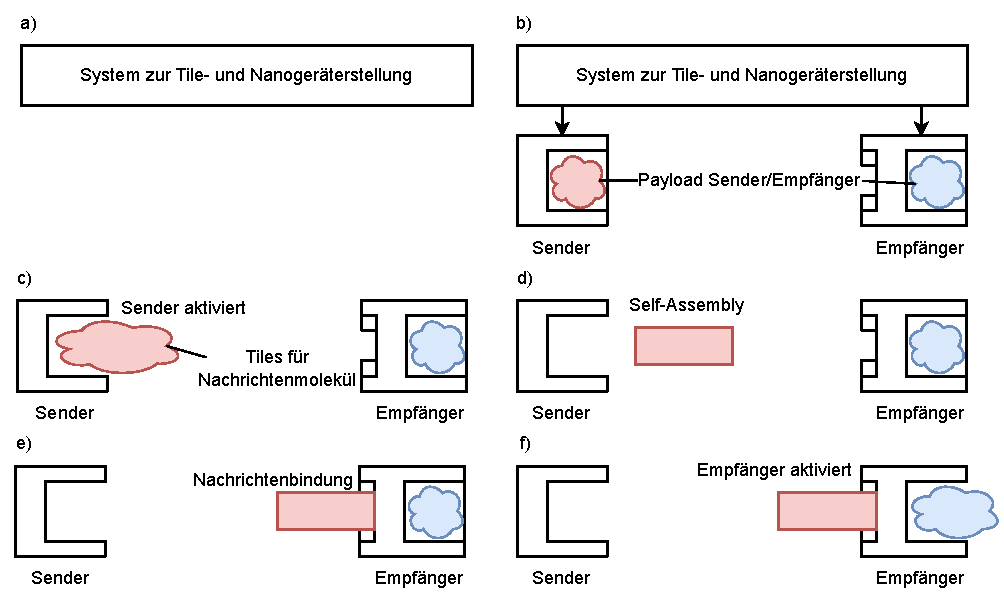
\includegraphics[width=\textwidth]{images/One-Way Communication.pdf}
    \caption[Einweg Kommunikation]{Skizzierte Darstellung einer Kommunikation von Nanogeräten, die nach dem Senden einer Nachricht aufgelöst oder aus dem System entfernt werden können. Dafür liegt in a) ein System zur Erstellung von Nanogeräten und Tiles vor. Dieses erstellt in b) den Sender und den Empfänger für den Kommunikationsschritt. Auch die Payloads beider Akteure werden durch das System gebildet. In c) werden die Tiles für die Self-Assembly durch die Aktivierung des Senders freigegeben. Diese Aktivierung kann durch unterschiedliche Mechanismen erfolgen. Das Binden von Liganden an Rezeptoren des Gerätes oder die Registrierung von Markern sind mögliche Mechanismen dafür. In d) wird das Nachrichtenmolekül durch Self-Assembly gebildet und in e) beim Empfänger gebunden. Dieser lässt daraufhin die Payload frei. Der Inhalt der Payload kann je nach Anwendungsfall unterschiedlich aussehen.}
    \label{fig:onewaycomm}
\end{figure}

\begin{figure}
    \centering
    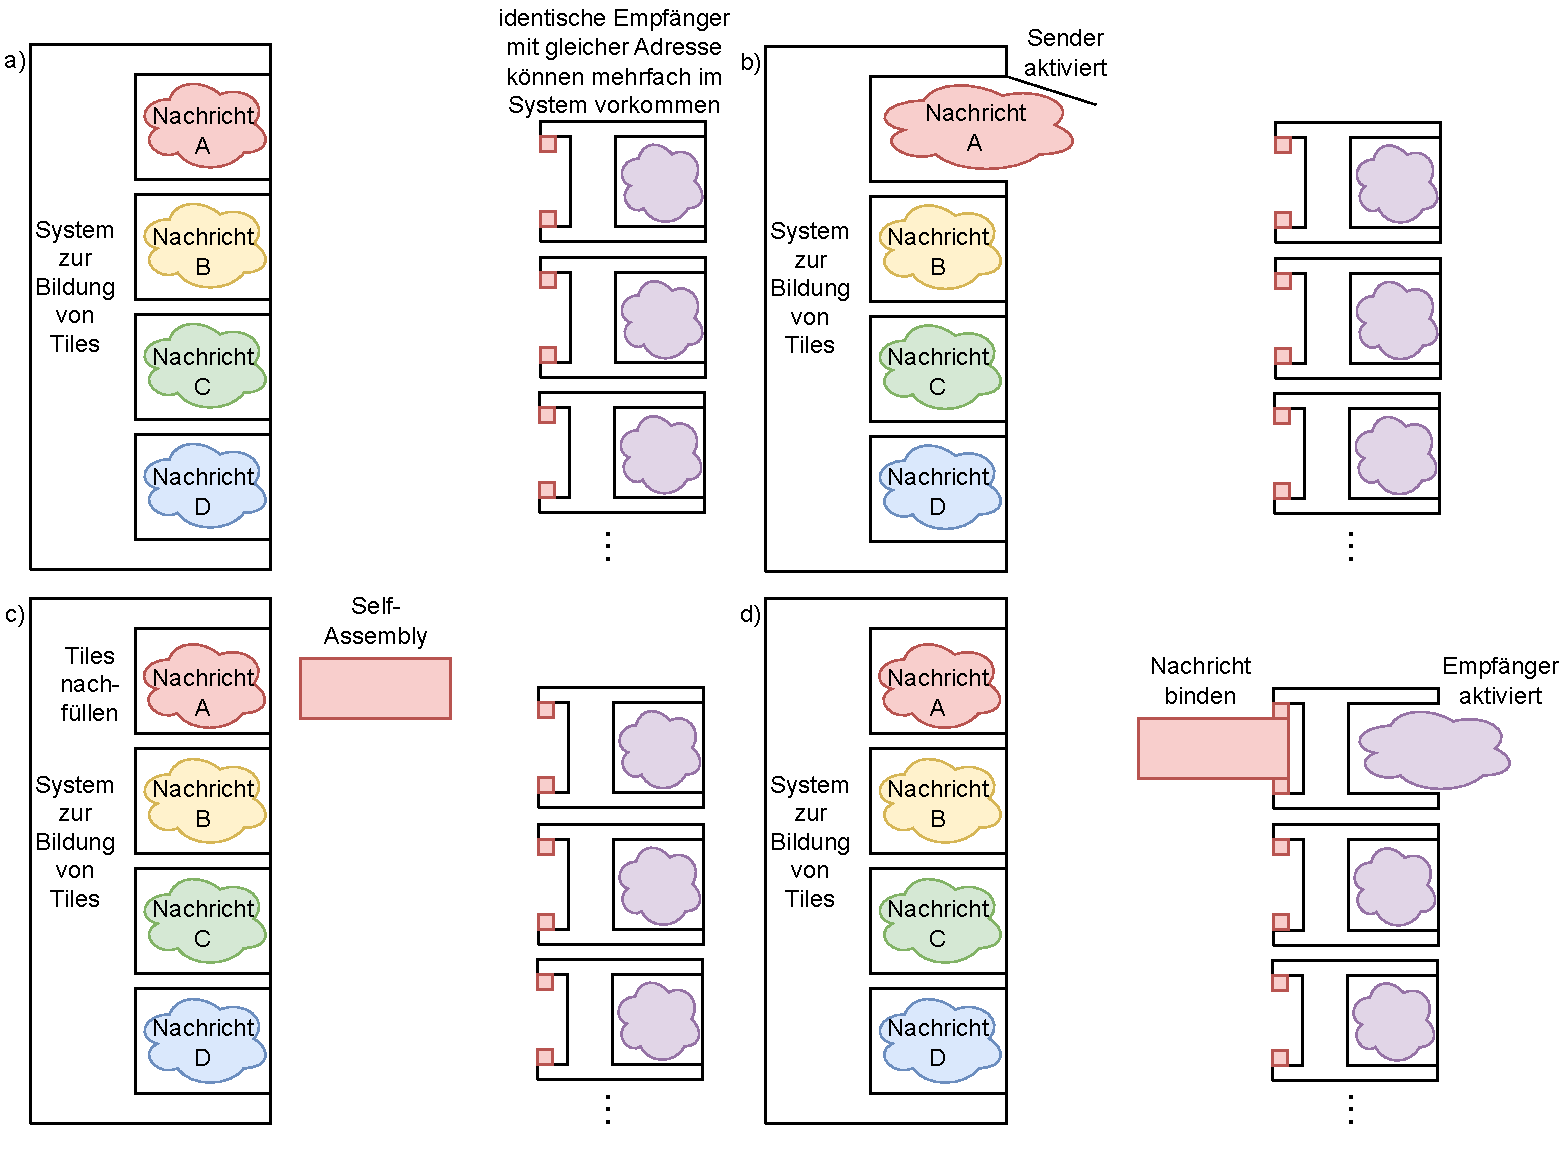
\includegraphics[width=\textwidth]{images/Multi-Way-Communication2.pdf}
    \caption[Mehrweg Kommunikation]{Skizzierte Darstellung einer Kommunikation von Nanogeräten, die erneutes Senden unterschiedlicher Nachrichten ermöglicht. In a) ist das System vorgestellt, welches das wiederholte Senden von Nachrichten ermöglicht. In b) wird das Nanogerät aktiviert, sodass eine Tileset freigelassen wird. Die Aktivierung kann durch unterschiedliche Mechanismen erfolgen. Eine Möglichkeit ist die Markererkennung oder die Bindung von Liganden an Rezeptoren. In c) kommt es zur Self-Assembly. Auch wird gezeigt, dass in so einem System die gleiche Nachricht erneut gesendet werden kann. In d) bindet sich die Nachricht beim Empfänger und dieser wird aktiviert. Damit kann beispielsweise die Payload des Empfängers freigelassen werden.}
    \label{fig:multiwaycomm}
\end{figure}

\section{Datenflusskontrolle durch Acknowledgements in Nanonetzwerken}

Der erste vorgestellte Mechanismus behandelt gleich drei der betrachteten Anforderungen an Datenflusskontrolle: die Vermeidung der Überlastung des Systems, die Effizienz und die Fehlerbehandlung.
Für Acknowledgements sind einige Faktoren interessant. Neben der Lebensdauer eines DNA-Moleküls im System $t_{deg}$ sind hier noch zwei weitere Angaben relevant. Die durchschnittliche Dauer zur Bildung eines Nachrichtenmoleküls durch Self-Assembly $t_{sa}(\tau,n)$. Diese ist abhängig von Temperatur $\tau$ des Systems und der Größe $n$ des Moleküls. Die Größe des Moleküls lässt sich dabei aus der Menge der Tiles bestimmen, die zur Konstruktion des gesamten Nachrichtenmoleküls verbunden werden. Der zweite wichtige Parameter ist die durchschnittliche Dauer des Bindens eines kompletten Moleküls nach Self-Assembly mit dem Empfänger des Nachrichtenmoleküls $t_{bind}$.

Um die Überlastung zu verringern, werden weitere Tilesets in den Prozess der Kommunikation verwendet. 
Ein Empfänger lässt beim Binden des Nachrichtenmoleküls ein solches Tileset frei. In Abbildung~\ref{fig:acks} sind zwei mögliche Self-Assemblies zu erkennen. Diese Assemblies stellen Acknowledgements dar, die schnellstmöglich gebildet und beim Sender gebunden werden, um den Erhalt der initialen Nachricht zu bestätigen. 
Dafür kann das Acknowledgement für ein möglichst kleines Molekül wie in Abbildung~\ref{fig:acks} a) nur aus einem Seed-Tile und einem Tile für die Liganden bestehen, der die Adressierung bestimmt. Eine andere Möglichkeit ist, dass es aus neun Tiles wie in Abbildung~\ref{fig:acks} b) besteht. 

Das Acknowledgement ist in diesen beiden Assemblies durch $\sigma_x$ und $K_x$ mit einen Index $x$ dargestellt. Dieser beschreibt die Notwendigkeit von eindeutigen Acknowledgements für jeden Kommunikationsvorgang. 
Es muss verhindert werden, dass ein Sender ein Acknowledgement einer vergangenen Nachricht verspätet erhält und sie für das Acknowledgement des zuletzt geschickten Nachrichtenmoleküls hält.
Das geschieht nur unter der Annahme, dass $t_{deg}$ groß genug gewählt ist. Somit können Assemblies und Tiles über mehrere Kommunikationsvorgänge nicht aus dem System entfernt werden. 
Somit benötigt jedes Acknowledgement einen eindeutigen Bezeichner, der je nach Kontext unterschiedlich festgelegt werden kann.
Die Assemblies in Abbildung~\ref{fig:acks} sind dabei nur Beispiele für Acknowledgements. In b) ist das Molekül zwar größer, jedoch kann dies je nach Anwendungsfall notwendig sein.
Ein anderer Ansatz für ein minimales Acknowledgement wie in a) könnte ein einzelnes Tile sein, welches sowohl Ligand als auch Seed-Assembly ist. 

\begin{figure}
    \centering
    \begin{tikzpicture}
        % Big ACK
        \node at (-1.2,2.3) {b)};
        \tileBigACKA{0}{1.2}
        \tileBigACKSigma{0}{0}
        \tileBigACKD{0}{-1.2}
        %
        \tileBigACKB{-1.2}{1.2}
        \tileBigACKKx{-1.2}{0}
        \tileBigACKE{-1.2}{-1.2}
        %
        \tileBigACKC{-2.4}{1.2}
        \tileBigACKM{-2.4}{0}
        \tileBigACKF{-2.4}{-1.2}
        % Small ACK
        \node at (-6.6,2.3) {a)};
        \tileSmallACKSigmax{-6}{0}
        \tileSmallACKA{-7.2}{0}
    \end{tikzpicture}
    \caption[Acknowledgements Tiles und Moleküle]{Darstellung von möglichen Acknowledgement Molekülen. In a) der Molekülhöhe eins und in b) der Molekülhöhe drei. Andere Größen und Formen für Acknowledgements sind denkbar und werden im Kapitel~\ref{cha:simulationen} näher betrachtet. Hier sind zwei Beispiele zur Veranschaulichung dargestellt.}
    \label{fig:acks}
\end{figure}

Es kann im Folgenden angenommen werden, dass ein Mechanismus im System existiert, der Acknowledgements nach dem Empfang der Nachricht freilässt. Dieses Nachrichtenmolekül kann sich dann beim Sender binden und gibt so die Bestätigung der erfolgreichen Übertragung. Auf dieser Basis kann Datenflusskontrolle durchgeführt werden.

Ein Sender lässt das Tileset für ein Nachrichtenmolekül frei. Für eine beliebige Übertragung und deren Dauer $t_{trans}$ gilt: Sei ein Nachrichtenmolekül der Größe $n$, bei einer Systemtemperatur $\tau$ und einem je nach Anwendung gewähltem Zeitpolster $t_w$ gegeben, kann folgendes betrachtet werden:
\begin{align*}
    \text{Neuübertragung}
    \begin{cases}
        \text{ja, } &\text{wenn } \lnot ACK \land t_{trans} > 2*(t_{sa}(\tau,n) + t_{bind}) + t_w\\
        \text{nein, } &\text{sonst }
    \end{cases}
\end{align*}

Dabei wird betrachtet, unter welchen Umständen es zu einer Neuübertragung kommt. Wenn innerhalb des durchschnittlichen Übertragungszeitraums zuzüglich eines Zeitpolsters kein Acknowledgement empfangen wird, erfolgt eine Neuübertragung.
Das Zeitpolster $t_w$ muss dabei so gewählt sein, dass nach Möglichkeit keine False-Positives für eine Neuübertragung entstehen. 
Dabei wird angenommen, dass das Sendermolekül größer ist als das Acknowledgement. Ist dies nicht der Fall, so muss $t_{sa}$ für das größere der beiden Moleküle betrachtet werden.

Durch diesen Mechanismus wird verhindert, dass ein langsamer Empfänger von einem schnellen Sender überlastet wird. Eine Optimierung der Zeitfenster steigert zudem die Effizienz, indem sie schnelle Neuübertragungen ermöglicht. Auch werden verlorene Nachrichten durch einen solchen Mechanismus erkannt und können durch die Neuübertragung wiederholt werden. Damit sind mit der Fehlerbehandlung drei der betrachteten Anforderungen an die Datenflusskontrolle vorgestellt. Im Folgenden soll der Aspekt der Gerechtigkeit im Medium betrachtet werden.

\section{Datenflusskontrolle durch Prioritätslevel in Nanonetzwerken}

\begin{table}
    \centering
    \begin{tabular}{l|l|l}
        & & Erlaubte Übertragung \\
        Priorität & Beispielhafter Nachrichtentyp & pro $t_{deg}$ Zyklus \\\hline 
        1 & Notfallbenachrichtigung & $\infty$ \\
        2 & Anweisung zur Medikamentausschüttung & $5$ \\
        3 & spezifische Werte anfragen & $3$ \\
        4 & allgemeiner Check & $1$
    \end{tabular}
    \caption[Prioritäten Beispiel]{Beispielhafte Einteilung von Nachrichtentypen in verschiedene Prioritätslevel für ein medizinischen System. Allen Prioritätsleveln wird aus Gerechtigkeitsgründen eine erlaubte Menge an Übertragungen pro Zyklus zugeteilt. Ein Zyklus stellt dabei die Zeitspanne $t_{deg}$ dar, welche die durchschnittliche Dauer des Verfalls oder Entfernung eines Tiles im Medium darstellt.}
    \label{tab:prio_gerechtigkeit}
\end{table}

Die Gerechtigkeit ist ein weiterer Faktor der Datenflusskontrolle. Dabei soll sichergestellt werden, dass alle Agierenden im Netzwerk regelmäßigen Zugriff auf das Medium erhalten. In einem Nanonetzwerk ist es jedoch schwierig, ohne Overhead einen Überblick darüber zu gewinnen, wer welche Nachrichten verschickt hat. Eine Lösung wäre es, durch ein zentrales Steuermedium verschiedene \emph{Prioritätslevel} für verschiedene Nachrichtentypen festzulegen. Dies ist beispielhaft in Tabelle~\ref{tab:prio_gerechtigkeit} für den Kontext In-Body-Networks dargestellt. Im Beispiel aus dieser Tabelle werden spezifischen Nachrichten eine höhere Priorität gegeben. Diese können unendlich oft oder mehrfach während eines $t_{deg}$ Zeitfensters übertragen werden. Nachrichten von niedriger Priorität jedoch nur wenige Male oder nur einmal. Durch einen solchen Mechanismus kann keine Gerechtigkeit garantiert werden, jedoch kann so verhindert werden, dass Beteiligte im Netzwerk das Medium mit \glqq unwichtigen\grqq\, Nachrichten flutet.

Dabei ist wichtig zu betonen, dass dieser Mechanismus vor allem dann von Bedeutung ist, wenn angenommen wird, dass das Medium in einem DNA-Tile-basierten Nanonetzwerk überflutet werden kann. Eine Stärke dieser Technologie ist ihre inhärente Parallelität: bei korrekt definierten Tilesets können mehrere Self-Assemblies simultan im selben Medium ablaufen, ohne Fehler zu verursachen. Dennoch könnte es Systeme geben, in denen ein Mechanismus zur Gerechtigkeit im Medium wichtig ist: beispielweise bei einer zentralen Steuerung, die durch eine Vielzahl von Nachrichten überlastet werden könnte. Daher kann ein Gerechtigkeitsmechanismus im Medium in bestimmten Anwendungsfällen durchaus sinnvoll sein.

Da einige Aspekte der Datenflusskontrolle mit Acknowledgements und Prioritätsleveln abgedeckt sind, kann mit der nächsten Anforderung weiter gemacht werden. 

\section{Nachrichtencodierung in Nanonetzwerken}
\label{sec:message_code}

Die nächste betrachtete Anforderung lässt sich schwer auf einzelne Anforderungen aus Kommunikationsprotokollen abbilden. Dabei geht es um die Darstellung von Nachrichten auf der Nanoebene. So wie in anderen Systemen müssen bei der Kommunikation in Nanonetzwerken Nachrichten zwischen Geräten verschickt werden. Diese werden durch Self-Assembly gebildet und durch die Bindung zwischen Liganden und Rezeptoren empfangen. Dabei muss das Nanogerät, das die Nachricht bindet, eine beliebige Nachricht $x$ von einer anderen Nachricht $y$ unterscheiden können.

Dafür soll in dieser Sektion eine Möglichkeit geliefert werden, mit welcher eine beliebige Anzahl an Nachrichten in einem System durch Tilesets und deren Self-Assembly gebildet werden können. Dabei liegt der Fokus darauf, die Nachrichtenmoleküle möglichst klein zu halten, ohne dabei zu große Tilesets zu erstellen. Die genaue Gewichtung dieser beiden Faktoren wird in Kapitel~\ref{cha:konstruktion} diskutiert.

Zur Codierung von Nachrichten auf Nanonetzwerkebene werden zwei Möglichkeiten vorgestellt: die Kodierung in den Kleberbezeichnern und die Kodierung in den Tilebezeichnern.
Wie beim Thema der Adressierung beschrieben wurde, können offene DNA-Stränge zur Informationskodierung verwendet werden. Somit ist auch die Informationskodierung in Kleberbezeichnern möglich.
Wenn die Information nicht in den Kleberbezeichnern codiert wird, kann sie auch in den Tilebezeichnern codiert werden. 

Dabei spielt die Struktur der gebildeten Tiles die entscheidende Rolle für die Codierung, nicht die offenen DNA-Enden.
Beispiele für beide Codierungsarten sind in Abbildung~\ref{fig:kodierung_glues} und Abbildung~\ref{fig:kodierung_label} gegeben. Beide Beispiele zeigen im Beispiel b) eine Self-Assembly für die Hexadezimalzahl \texttt{ab1}. In Abbildung~\ref{fig:kodierung_glues} sind in a) alle Tiles zu sehen, die zur Codierung von dreistelligen Hexadezimalzahlen in den Kleberbezeichnern benötigt werden. Insgesamt 100 Tiles sind notwendig und die finale Self-Assembly besteht aus zehn Tiles. Es ist möglich zwei Tiles im Tileset und der Self-Assembly zu sparen, indem die Liganden mit den Bezeichnern \glqq Z\grqq\, und \glqq K\grqq\, entfernt werden. Dann müssten alle Tiles mit den Bezeichnern \glqq Y\grqq\, und \glqq J\grqq\ die Liganden bilden. Somit würde das Tileset 98 Tiles umfassen und die Self-Assembly acht Tiles. Aus Gründen der Übersichtlichkeit wurde dies im Beispiel aus Abbildung~\ref{fig:kodierung_glues} nicht getan. Das Prinzip wird jedoch im Beispiel aus Abbildung~\ref{fig:kodierung_label} angewendet. Auch hier sind in a) alle Tiles dargestellt, die zur Codierung einer dreistelligen Hexadezimalzahl benötigt werden. In b) ist die beispielhafte Self-Assembly zu sehen. Dieser Ansatz benötigt 48 Tiles im Tileset und vier Tiles in der Self-Assembly. Wird angenommen, dass auch hier die Liganden in einzelnen Tiles gebildet werden, verändert sich das leicht. Dabei wäre das Tileset 49 Tiles und die Assembly fünf Tiles groß.

\begin{figure}
    \centering
    \begin{tikzpicture}[scale = 0.9]
        % Sigma/V/K/Z-Tile
        \node at (-1,-7.5) {a)};
        \tileCodeGluesSigma{0}{0}
        \tileCodeGluesV{1.5}{0}
        \tileCodeGluesK{3}{0}
        \tileCodeGluesZ{4.5}{0}
        % Row 1
        \tileCodeGluesWNull{0}{-1.5}
        \tileCodeGluesWEins{1.5}{-1.5}
        \tileCodeGluesWZwei{3}{-1.5}
        \tileCodeGluesWDrei{4.5}{-1.5}
        \tileCodeGluesWVier{6}{-1.5}
        \tileCodeGluesWFuenf{7.5}{-1.5}
        \tileCodeGluesWSechs{9}{-1.5}
        \tileCodeGluesWSieben{10.5}{-1.5}
        \tileCodeGluesWAcht{12}{-1.5}
        \tileCodeGluesWNeun{13.5}{-1.5}
        % Row 2
        \tileCodeGluesWA{0}{-3}
        \tileCodeGluesWB{1.5}{-3}
        \tileCodeGluesWC{3}{-3}
        \tileCodeGluesWD{4.5}{-3}
        \tileCodeGluesWE{6}{-3}
        \tileCodeGluesWD{7.5}{-3}
        \tileCodeGluesXNull{9}{-3}
        \tileCodeGluesXEins{10.5}{-3}
        \tileCodeGluesXZwei{12}{-3}
        \tileCodeGluesXDrei{13.5}{-3}
        % Row 3
        \tileCodeGluesXVier{0}{-4.5}
        \tileCodeGluesXFuenf{1.5}{-4.5}
        \tileCodeGluesXSechs{3}{-4.5}
        \tileCodeGluesXSieben{4.5}{-4.5}
        \tileCodeGluesXAcht{6}{-4.5}
        \tileCodeGluesXNeun{7.5}{-4.5}
        \tileCodeGluesXA{9}{-4.5}
        \tileCodeGluesXB{10.5}{-4.5}
        \tileCodeGluesXC{12}{-4.5}
        \tileCodeGluesXD{13.5}{-4.5}
        % Row 4
        \tileCodeGluesXE{0}{-6}
        \tileCodeGluesXF{1.5}{-6}
        \tileCodeGluesYNull{3}{-6}
        \tileCodeGluesYEins{4.5}{-6}
        \tileCodeGluesYZwei{6}{-6}
        \tileCodeGluesYDrei{7.5}{-6}
        \tileCodeGluesYVier{9}{-6}
        \tileCodeGluesYFuenf{10.5}{-6}
        \tileCodeGluesYSechs{12}{-6}
        \tileCodeGluesYSieben{13.5}{-6}
        % Row 5
        \tileCodeGluesYAcht{0}{-7.5}
        \tileCodeGluesYNeun{1.5}{-7.5}
        \tileCodeGluesYA{3}{-7.5}
        \tileCodeGluesYB{4.5}{-7.5}
        \tileCodeGluesYC{6}{-7.5}
        \tileCodeGluesYD{7.5}{-7.5}
        \tileCodeGluesYE{9}{-7.5}
        \tileCodeGluesYF{10.5}{-7.5}
        \tileCodeGluesHNull{12}{-7.5}
        \tileCodeGluesHEins{13.5}{-7.5}
        % Row 6
        \tileCodeGluesHZwei{0}{-9}
        \tileCodeGluesHDrei{1.5}{-9}
        \tileCodeGluesHVier{3}{-9}
        \tileCodeGluesHFuenf{4.5}{-9}
        \tileCodeGluesHSechs{6}{-9}
        \tileCodeGluesHSieben{7.5}{-9}
        \tileCodeGluesHSieben{9}{-9}
        \tileCodeGluesHAcht{10.5}{-9}
        \tileCodeGluesHNeun{12}{-9}
        \tileCodeGluesHA{13.5}{-9}
        % Row 7
        \tileCodeGluesHB{0}{-10.5}
        \tileCodeGluesHC{1.5}{-10.5}
        \tileCodeGluesHD{3}{-10.5}
        \tileCodeGluesHE{4.5}{-10.5}
        \tileCodeGluesHF{6}{-10.5}
        \tileCodeGluesINull{7.5}{-10.5}
        \tileCodeGluesIEins{9}{-10.5}
        \tileCodeGluesIZwei{10.5}{-10.5}
        \tileCodeGluesIDrei{12}{-10.5}
        \tileCodeGluesIVier{13.5}{-10.5}
        % H-Tiles Row 2
        \tileCodeGluesIFuenf{0}{-12}
        \tileCodeGluesISechs{1.5}{-12}
        \tileCodeGluesISieben{3}{-12}
        \tileCodeGluesIAcht{4.5}{-12}
        \tileCodeGluesINeun{6}{-12}
        \tileCodeGluesIA{7.5}{-12}
        \tileCodeGluesIB{9}{-12}
        \tileCodeGluesIC{10.5}{-12}
        \tileCodeGluesID{12}{-12}
        \tileCodeGluesIE{13.5}{-12}
        % Row 8
        \tileCodeGluesIF{0}{-13.5}
        \tileCodeGluesJNull{1.5}{-13.5}
        \tileCodeGluesJEins{3}{-13.5}
        \tileCodeGluesJZwei{4.5}{-13.5}
        \tileCodeGluesJDrei{6}{-13.5}
        \tileCodeGluesJVier{7.5}{-13.5}
        \tileCodeGluesJFuenf{9}{-13.5}
        \tileCodeGluesJSechs{10.5}{-13.5}
        \tileCodeGluesJSieben{12}{-13.5}
        \tileCodeGluesJAcht{13.5}{-13.5}
        % Row 9
        \tileCodeGluesJA{0}{-15}
        \tileCodeGluesJB{1.5}{-15}
        \tileCodeGluesJC{3}{-15}
        \tileCodeGluesJD{4.5}{-15}
        \tileCodeGluesJE{6}{-15}
        \tileCodeGluesJF{7.5}{-15}
        %%%% 
        % Bsp. Assembly Row 1
        \draw[line width=1pt] (-0.6,-16) -- (14.1,-16);
        \node at (-1,-17.8) {b)};
        \tileCodeGluesZ{0}{-17.2}
        \tileCodeGluesYA{1.2}{-17.2}
        \tileCodeGluesXB{2.4}{-17.2}
        \tileCodeGluesWEins{3.6}{-17.2}
        \tileCodeGluesV{4.8}{-17.2}
        % Bsp. Assembly Row 2
        \tileCodeGluesK{0}{-18.4}
        \tileCodeGluesJA{1.2}{-18.4}
        \tileCodeGluesIB{2.4}{-18.4}
        \tileCodeGluesHEins{3.6}{-18.4}
        \tileCodeGluesSigma{4.8}{-18.4}
        \draw[line width=1.5pt, green] (0.9,-18.2) rectangle (3.9,-17.4);
    \end{tikzpicture}
    \caption[Dreistellige Hexadezimalzahl in den Kleberbezeichnern codiert]{Beispielhafte Codierung der dreistelligen Hexadezimalzahl \texttt{ab1} (grün), wobei die Codierung in den Kleberbezeichnern stattfindet. In a) ist dafür das Tileset für alle notwendigen Tiles zur Codierung einer dreistelligen Hexadezimalzahl in den Kleberbezeichnern abgebildet. In b) ist die Self-Assembly für die Hexadezimalzahl \texttt{ab1} abgebildet.}
    \label{fig:kodierung_glues}
\end{figure}

Wird bei beiden Ansätzen davon ausgegangen, dass sie den Beispielen aus den Abbildungen \ref{fig:kodierung_glues} und \ref{fig:kodierung_label} folgen, dann lässt sich für eine Zahl im Basis-$x$-System und der Anzahl der Ziffern $y$ Folgendes sagen:
Wird die Zahl in den Kleberbezeichnern codiert, so hat das Tileset $2xy + 4$ Tiles und die Self-Assembly $2y+4$ Tiles.
Wird die Zahl in einem einzelnen Tile codiert, dann hat das Tileset $yx+1$ Tiles und die Self-Assembly $y+1$ Tiles.
In den Beispielen aus Abbildungen \ref{fig:kodierung_glues} und \ref{fig:kodierung_label} liegt eine Hexadezimalzahl mit drei Ziffernstellen vor. Somit lässt sich beispielsweise für Kleberbezeichner $2\cdot 16\cdot 3+4 = 100$ berechnen.
Für sowohl die Größe der Self-Assembly als auch für die Größe des benötigten Tilesets kann erkannt werden, dass die Codierung in den Bezeichnern des Tiles effizienter ist, da jede Ziffer eines beliebigen Zahlensystems durch ein statt zwei Tiles dargestellt werden kann.

Jedoch muss dabei betrachtet werden, dass die Tilebezeichner auf der mathematischen Ebene verwendet werden, damit Nutzer*innen des Systems eine bessere Übersicht über die verschiedenen Tiles haben. 
Um darin die Codierung durchzuführen, muss ein neuer Ansatz gefunden werden, der diese Bezeichner auch im praktischen Anwendungsfall ermöglicht. 
Ein Vorschlag dafür ist die interne Struktur des Tiles zu verwenden, um Bezeichner zu realisieren. 
Die DNA-Basenpaare im Inneren des Tiles können so analysiert und spezifisch für einen Bezeichner verwendet werden.

\begin{figure}
    \centering
    \begin{tikzpicture}[scale=0.9]
        % Sigma-Tile
        \node at (-1,-3.75) {a)};
        \tileCodeLabelSigma{0}{0}
        % X-Tiles Row 1
        \tileCodeLabelXNull{0}{-1.5}
        \tileCodeLabelXEins{1.5}{-1.5}
        \tileCodeLabelXZwei{3}{-1.5}
        \tileCodeLabelXDrei{4.5}{-1.5}
        \tileCodeLabelXVier{6}{-1.5}
        \tileCodeLabelXFuenf{7.5}{-1.5}
        \tileCodeLabelXSechs{9}{-1.5}
        \tileCodeLabelXSieben{10.5}{-1.5}
        \tileCodeLabelXAcht{12}{-1.5}
        \tileCodeLabelXNeun{13.5}{-1.5}
        % X-Tiles Row 2
        \tileCodeLabelXA{0}{-3}
        \tileCodeLabelXB{1.5}{-3}
        \tileCodeLabelXC{3}{-3}
        \tileCodeLabelXD{4.5}{-3}
        \tileCodeLabelXE{6}{-3}
        \tileCodeLabelXF{7.5}{-3}
        \tileCodeLabelYNull{9}{-3}
        \tileCodeLabelYEins{10.5}{-3}
        \tileCodeLabelYZwei{12}{-3}
        \tileCodeLabelYDrei{13.5}{-3}
        % Y-Tiles Row 1
        \tileCodeLabelYVier{0}{-4.5}
        \tileCodeLabelYFuenf{1.5}{-4.5}
        \tileCodeLabelYSechs{3}{-4.5}
        \tileCodeLabelYSieben{4.5}{-4.5}
        \tileCodeLabelYAcht{6}{-4.5}
        \tileCodeLabelYNeun{7.5}{-4.5}
        \tileCodeLabelYA{9}{-4.5}
        \tileCodeLabelYB{10.5}{-4.5}
        \tileCodeLabelYC{12}{-4.5}
        \tileCodeLabelYD{13.5}{-4.5}
        % Y-Tiles Row 2
        \tileCodeLabelYE{0}{-6}
        \tileCodeLabelYF{1.5}{-6}
        \tileCodeLabelZEins{3}{-6}
        \tileCodeLabelZZwei{4.5}{-6}
        \tileCodeLabelZDrei{6}{-6}
        \tileCodeLabelZVier{7.5}{-6}
        \tileCodeLabelZFuenf{9}{-6}
        \tileCodeLabelZSechs{10.5}{-6}
        \tileCodeLabelZSieben{12}{-6}
        \tileCodeLabelZAcht{13.5}{-6}
        % Z-Tiles Row 1
        \tileCodeLabelZNeun{0}{-7.5}
        \tileCodeLabelZA{1.5}{-7.5}
        \tileCodeLabelZB{3}{-7.5}
        \tileCodeLabelZC{4.5}{-7.5}
        \tileCodeLabelZD{6}{-7.5}
        \tileCodeLabelZE{7.5}{-7.5}
        \tileCodeLabelZF{9}{-7.5}
        %%%% 
        % Bsp. Assembly Row 1
        \draw[line width=1pt] (-0.6,-8.5) -- (14.1,-8.5);
        \node at (-1,-9.5) {b)};
        \tileCodeLabelZA{0}{-9.5}
        \tileCodeLabelYB{1.2}{-9.5}
        \tileCodeLabelXEins{2.4}{-9.5}
        \tileCodeLabelSigma{3.6}{-9.5}
        \draw[line width=1.5pt, green] (-0.3,-9.3) rectangle (2.6,-9.7);
    \end{tikzpicture}
    \caption[Dreistellige Hexadezimalzahl in den Tile Bezeichnern codiert]{Beispielhafte Codierung der dreistelligen Hexadezimalzahl \texttt{ab1} (grün), wobei die Codierung in den Tilebezeichnern stattfindet. In a) ist dafür das Tileset für alle notwendigen Tiles zur Codierung einer dreistelligen Hexadezimalzahl in den Tilebezeichnern abgebildet. In b) ist die Self-Assembly für die Hexadezimalzahl \texttt{ab1} abgebildet.}
    \label{fig:kodierung_label}
\end{figure}

Wenn in einem Nanonetzwerk eine beliebige Anzahl unterschiedlicher Nachrichten vorhanden ist, können diese in ein entsprechendes Zahlensystem übertragen werden. Als Beispiel dient dabei wieder das In-Body-Network. Gibt es im Netzwerk beispielsweise 20 unterschiedliche Kontrollnachrichten und 200 verschiedene Krankheitsbilder, die durch Nachrichten übermittelt werden sollen, so ergibt das insgesamt 220 Nachrichten. Mit einer zweistelligen Hexadezimalzahl könnten 256 Nachrichten codiert werden, wofür 33 Tiles für das Tileset und drei Tiles für die Self-Assembly benötigt werden.

Sollte das Netzwerk jedoch 300 verschiedene Krankheitsbilder unterstützen, wäre eine zweistellige Hexadezimalzahl unzulänglich.
Obwohl eine dreistellige Hexadezimalzahl die Kapazität hat, ist es ineffizient, eine Zahl zu wählen, die 4096 Nachrichten kodieren kann. Dabei werden 49 Tiles im Tileset und vier Tiles in der Self-Assembly benötigt. Da nur 320 Nachrichten kodiert werden müssen, sollte ein kleineres Zahlensystem gewählt werden. Ein effizienterer Ansatz wäre die Verwendung einer dreistelligen Oktalzahl. Hierbei würden 25 Tiles für das Tileset und vier Tiles für die Self-Assembly ausreichen, um 320 Nachrichten zu kodieren.

Die Entscheidung für das optimale Zahlensystem hängt von der Gewichtung zwischen der Größe der Self-Assembly und der Größe des Tilesets ab. Wird die Tilebezeichner-Codierung verwendet, sollte das Zahlensystem so gewählt werden, dass die Ergebnisse der Formeln $xy+1$ und $y+1$ (für $y$-stellige Zahl der Basis $x$) möglichst gering sind. Werden diesen Formeln spezifische Gewichtungen zugewiesen, kann das Auswahlverfahren durch den folgenden Pseudocode repräsentiert werden:


\begin{lstlisting}[language=Python, caption={[Pseudocode für eine Funktion zur Definition der besten Basis.]{Pseudocode für eine Funktion zur Definition der besten Basis abhängig von der Anzahl der zu codierenden Nachrichten und den Gewichtungen von Tileset und Assembly. Der gesamte Code ist im Anhang \ref{app:code} verlinkt.}}, label=lst:best_base]
# m = Anzahl der Nachrichten die codiert werden muss
# w1 = Gewichtung Formel 1 (xy+1)
# w2 = Gewichtung Formel 2 (y+1)
def get_best_base(m, w1, w2):
    # initialisieren
    best_base = 2
    best_score = inf 
    best_f1 = 0
    best_f2 = 0

    for b in range(2, m+1)
        # bestimme Anzahl der Ziffern von m zur Basis b
        y = convert_m_to_base(m, b)
        f1 = b * y + 1
        f2 = y + 1
        score = w1 * f1 * w2 * f2
        # wenn der aktuelle Score kleiner ist, 
        # liegt effizientere Basis vor
        if score < best_score
            best_score = score 
            best_base = base 
            best_f1 = f1 
            best_f2 = f2
    return best_base, best_f1, best_f2
\end{lstlisting}

Die Gewichtung der Formeln kann beliebig gewählt werden. Ist die Gewichtung beispielsweise $w_1 = 1$ und $w_2 = 10$, so bedeutet dies, dass ein Tile in der Self-Assembly das gleiche Gewicht hat wie zehn Tiles im Tileset.

In dieser Sektion wurde für Erklärungszwecke vereinfacht angenommen, dass die Codierung von DNA-Tiles auf verschiedene Zahlensysteme trivial ist. Tatsächlich erfolgt die Codierung auf Nanoebene stets in der DNA-Sprache von \emph{ATCG}. Dafür wird angenommen, dass DNA analog auf Binärzahlen übertragen werden kann. So kann jedes \emph{AT} oder \emph{TA} Basenpaar beispielsweise binär als \texttt{0} und jedes Basenpaar \emph{CG} oder \emph{GC} binär als \texttt{1} codiert werden. Auch ein ein Zahlensystem der Basis vier ist denkbar, das die Reihenfolge der Basenpaare berücksichtigt.

Die Umwandlung von Binärzahlen in andere Zahlensysteme, wie Hexadezimalzahlen, kann ohne Overhead erfolgen. Beispielsweise lässt sich eine vierstellige Binärzahl direkt in eine Hexadezimalzahl übersetzen. Komplikationen ergeben sich jedoch, wenn man Binärzahlen in ein Dezimalsystem umwandeln möchte. Während eine vierstellige Binärzahl 16 Zahlen darstellen kann, ist eine dreistellige Binärzahl auf acht Zahlen beschränkt. Dies kann zu Overhead in der Codierung führen.

Da in dieser Arbeit das mathematische Tile-Modell betrachtet wird und die Codierung in den mathematischen Bezeichnern stattfindet, wird dies in der Arbeit nicht weiter betrachtet. Sollte der Mechanismus in einem Nanonetzwerk implementiert werden, muss darauf geachtet werden.  

Nach Auswahl des effizientesten Zahlensystems können Nachrichten mittels Preprocessing in das entsprechende System umgewandelt werden. Dies ermöglicht die Erstellung von Nachrichtenmolekülen mit minimaler Anzahl an Tiles und kleinstmöglichen Assemblies für das Netzwerk. Weiterhin ermöglicht das Preprocessing eine Optimierung der benötigten Nachrichtenanzahl. Einige Nachrichten könnten eventuell durch den Einsatz von Flags optimiert werden, die in der Sektion~\ref{sec:flags} näher erläutert werden.

\section{Self-Assemblies in ihrer Höhe anpassen}

Bevor mit weiteren Anforderungen fortgefahren wird, muss zunächst die Höhe von Self-Assemblies thematisiert werden. In dieser Arbeit werden verschiedene Self-Assemblies dargestellt, die unterschiedliche Höhen aufweisen. Eine Verringerung der Höhe einer Self-Assembly ist nicht immer möglich, da hierbei Informationen verloren gehen könnten. Das bislang verwendete Beispiel für den Äquivalenzvergleich aus Abbildung~\ref{fig:eq_bsp} kann beispielsweise nicht in eine Self-Assembly der Höhe zwei oder eins umgewandelt werden, ohne grundlegende Änderungen an der Struktur und Funktionsweise der Self-Assembly vorzunehmen.

Es ist jedoch trivial, die Höhe einer Self-Assembly zu erhöhen. Dies wird beispielhaft in Abbildung~\ref{fig:assembly_height} an einer Self-Assembly der Höhe eins gezeigt. Dabei müssen lediglich die Seed-Assembly und die Liganden angepasst werden. Der im Beispiel gezeigte Ligand wird zu einem Tile umfunktioniert, der die neu hinzugefügten Liganden bindet. Daher kann einer Self-Assembly der Höhe eins einfach ein Rahmen hinzugefügt werden, um ihre Höhe auf zwei oder drei zu erhöhen, ohne die eigentliche Information der Self-Assembly zu verändern.

\begin{figure}
    \centering 
    \begin{tikzpicture}
        \tileAssemblyHeightB{0}{0}
        \tileAssemblyHeightA{1.2}{0}
        \tileAssemblyHeightSigma{2.4}{0}
        %
        \node at (3.4,0) {$\Rightarrow$};
        %
        \tileAssemblyHeightBSmall{4.4}{0}
        \tileAssemblyHeightA{5.6}{0}
        \tileAssemblyHeightSigmaSmall{6.8}{0}
        %
        \tileAssemblyHeightZ{4.4}{-1.2}
        \tileAssemblyHeightY{5.6}{-1.2}
        \tileAssemblyHeightX{6.8}{-1.2}
        %
        \node at (7.8,0) {$\Rightarrow$};
        %
        \tileAssemblyHeightO{8.8}{1.2}
        \tileAssemblyHeightN{10}{1.2}
        \tileAssemblyHeightM{11.2}{1.2}
        %
        \tileAssemblyHeightBBig{8.8}{0}
        \tileAssemblyHeightA{10}{0}
        \tileAssemblyHeightSigmaBig{11.2}{0}
        %
        \tileAssemblyHeightZ{8.8}{-1.2}
        \tileAssemblyHeightY{10}{-1.2}
        \tileAssemblyHeightX{11.2}{-1.2}
        %\draw[line width=1pt] (-0.6,-3) -- (11,-3);
    \end{tikzpicture}
    \caption[Beispiel zur Vergrößerung einer Assembly]{Beispiel für das Anpassen der Höhe einer Assembly. Links ist dabei eine Self-Assembly der Höhe eins dargestellt. Diese kann durch Anpassung der Seed-Assembly und des Liganden zu einer Assembly der Höhe zwei (mittig) oder der Höhe drei (rechts) erweitert werden. Dabei verändert sich die Information der Self-Assembly selbst nicht. Nur die inneren Kleber beziehungsweise die Liganden verändern sich.}
    \label{fig:assembly_height}
\end{figure}

Dafür muss nur entweder der südliche oder nördliche Kleber von Seed-Assembly und Liganden angepasst werden. Dieser Mechanismus lässt sich für beliebige Höhen wiederholen. Dabei wird dann nicht die Seed-Assembly angepasst, sondern die Tiles nördlich und südlich der Seed-Assembly.

Mit dem beschriebenen Ansatz ist es möglich, für alle Self-Assemblies in einem System eine einheitliche Größe festzulegen. Dabei wird jedoch nicht betrachtet, ob der hinzugefügte Rahmen Informationen speichern kann, um die Effizienz der erweiterten Self-Assembly zu steigern. Dies muss individuell für jeden Fall betrachtet und neu implementiert werden. Mit diesem Verständnis über die Höhe von Self-Assemblies können nun die weiteren Anforderungen besprochen werden.

\section{Flags in Nanonetzwerken}
\label{sec:flags}
Flags werden in herkömmlichen Kommunikationsprotokollen verwendet, um bestimmte Eigenschaften oder Zustände einer Nachricht im Header zu kennzeichnen. Typische Flags sind beispielsweise Synchronisationsflags, welche in TCP verwendet werden, um einen Three-Way-Handshake zu signalisieren. Auch Acknowledgements werden in Flags verwendet, um zu signalisieren, dass das letzte Paket beim Empfänger angekommen ist. Die Finish-Flag zeigt an, dass es sich um die letzte Nachricht der Übertragung handelt, während die Reset-Flag zur abrupten Beendung einer Übertragung genutzt wird. 

Es können je nach Anwendungsfall verschiedene Flags verwendet werden. Die hier vorgestellten Flags lassen sich jedoch nicht sinnvoll auf Nanonetzwerkebene abstrahieren. Acknowledgements wurden im letzten Absatz beschrieben und können in einem offenen System als eigene Nachricht verschickt werden. In einem auf DNA und Self-Assembly basierten Nanonetzwerk, in welchem über Nachrichtenmolekülen zwischen zwei Entitäten kommuniziert wird und mehrere Nachrichten in einer Übertragung verschickt werden, könnten sich Acknowledgement-Flags anbieten. Davon wird in dieser Arbeit jedoch nicht ausgegangen. 

Synchronisation ist in Nanonetzwerken ein weiteres Problem. Dadurch, dass bei der Self-Assembly der Vorgang der Nachrichtenübertragung aus der Hand des Nutzers gegeben wird und sich alles auf dem sehr kleinen Skalenbereich der Nanoebene bewegt, lässt sich Zeit schwer synchronisieren. Es bietet sich allgemein an, asynchron zu kommunizieren. Ein Three-Way-Handshake oder andere Mechanismen, die eine relative Synchronisation zueinander ermöglichen, könnten eine Möglichkeit auf Nanoebene bieten. Dabei wird nicht die Zeit der Geräte synchronisiert, sondern ein relativer Zähler oder ein anderer Mechanismus verwendet, damit die kommunizierenden Geräte eine gemeinsam festgelegte Möglichkeit haben, um festzustellen, ob eine Nachricht verloren gegangen ist. Jedoch wurde in diesem Kapitel beschrieben, dass in Nanonetzwerken die Nachrichtenmenge minimalisiert werden soll und der Dialog von zwei Geräten über mehrere Nachrichten ungewöhnlich für Systeme auf dieser Skala ist. Somit wird für diese Arbeit asynchrone Kommunikation angenommen, da viele der Mechanismen außerhalb der Tile-basierten Self-Assembly durchgeführt werden müssten.
\begin{figure}
    \centering 
    \begin{tikzpicture}
        % Tileset Bsp 1
        \node at (-1,0) {a)};
        \tileFlagsHeigthOneC{0}{0}
        \tileFlagsHeigthOneD{1.5}{0}
        \tileFlagsHeigthOneE{3}{0}
        \tileFlagsHeigthOneSigmaAlt{4.5}{0}
        \tileFlagsHeigthOneFOne{7}{0}
        \tileFlagsHeigthOneFZero{8.5}{0}
        \tileFlagsHeigthOneSigma{10}{0}
        % Assembly Bsp 1
        \draw[line width=1pt] (-0.6,-1) -- (11,-1);
        \node at (-1,-2) {b)};
        \tileFlagsHeigthOneE{0}{-2}
        \tileFlagsHeigthOneD{1.2}{-2}
        \tileFlagsHeigthOneC{2.4}{-2}
        \tileFlagsHeigthOneSigmaAlt{3.6}{-2}
        \node at (4.6,-2) {$\Rightarrow$};
        \tileFlagsHeigthOneE{5.6}{-2}
        \tileFlagsHeigthOneD{6.8}{-2}
        \tileFlagsHeigthOneC{8}{-2}
        \tileFlagsHeigthOneFOne{9.2}{-2}
        \tileFlagsHeigthOneSigma{10.4}{-2}
        % Tileset Bsp 2
        \draw[line width=1pt] (-0.6,-3) -- (11,-3);
        \node at (-1,-5.5) {c)};
        \tileFlagsHeigthThreeSigma{0}{-4}
        \tileFlagsHeigthThreeC{1.5}{-4}
        \tileFlagsHeigthThreeD{3}{-4}
        \tileFlagsHeigthThreeE{4.5}{-4}
        %
        \tileFlagsHeigthThreeWAlt{0}{-5.5}
        \tileFlagsHeigthThreeX{1.5}{-5.5}
        \tileFlagsHeigthThreeY{3}{-5.5}
        \tileFlagsHeigthThreeZ{4.5}{-5.5}
        %
        \tileFlagsHeigthThreeMAlt{0}{-7}
        \tileFlagsHeigthThreeN{1.5}{-7}
        \tileFlagsHeigthThreeO{3}{-7}
        \tileFlagsHeigthThreeP{4.5}{-7}
        %%%%%%%%%
        \tileFlagsHeigthThreeFOne{7}{-4}
        \tileFlagsHeigthThreeFZero{8.5}{-4}
        %
        \tileFlagsHeigthThreeG{7}{-5.5}
        \tileFlagsHeigthThreeH{8.5}{-5.5}
        %
        \tileFlagsHeigthThreeW{7}{-7}
        \tileFlagsHeigthThreeM{8.5}{-7}
        % Assembly Bsp 2
        \draw[line width=1pt] (-0.6,-8) -- (11,-8);
        \node at (-1,-10.2) {d)};
        \tileFlagsHeigthThreeZ{0}{-9}
        \tileFlagsHeigthThreeE{0}{-10.2}
        \tileFlagsHeigthThreeP{0}{-11.4}
        %
        \tileFlagsHeigthThreeY{1.2}{-9}
        \tileFlagsHeigthThreeD{1.2}{-10.2}
        \tileFlagsHeigthThreeO{1.2}{-11.4}
        %
        \tileFlagsHeigthThreeX{2.4}{-9}
        \tileFlagsHeigthThreeC{2.4}{-10.2}
        \tileFlagsHeigthThreeN{2.4}{-11.4}
        %
        \tileFlagsHeigthThreeWAlt{3.6}{-9}
        \tileFlagsHeigthThreeSigma{3.6}{-10.2}
        \tileFlagsHeigthThreeMAlt{3.6}{-11.4}
        %
        \node at (4.6,-10.2) {$\Rightarrow$};
        %
        \tileFlagsHeigthThreeZ{5.6}{-9}
        \tileFlagsHeigthThreeE{5.6}{-10.2}
        \tileFlagsHeigthThreeP{5.6}{-11.4}
        %
        \tileFlagsHeigthThreeY{6.8}{-9}
        \tileFlagsHeigthThreeD{6.8}{-10.2}
        \tileFlagsHeigthThreeO{6.8}{-11.4}
        %
        \tileFlagsHeigthThreeX{8}{-9}
        \tileFlagsHeigthThreeC{8}{-10.2}
        \tileFlagsHeigthThreeN{8}{-11.4}
        %
        \tileFlagsHeigthThreeG{9.2}{-9}
        \tileFlagsHeigthThreeFOne{9.2}{-10.2}
        \tileFlagsHeigthThreeH{9.2}{-11.4}
        %
        \tileFlagsHeigthThreeW{10.4}{-9}
        \tileFlagsHeigthThreeSigma{10.4}{-10.2}
        \tileFlagsHeigthThreeM{10.4}{-11.4}
    \end{tikzpicture}
    \caption[Flags Beispiel]{Darstellung der Erweiterung von Self-Assembly Molekülen durch Flagtiles. In a) und c) sind die jeweiligen Tilesets links dargestellt. Rechts sind jeweils die Tiles dargestellt, die entweder überarbeitet (bei gleichem Bezeichner) oder neu hinzugefügt werden müssen, um Flags zu implementieren. In b) und d) sind jeweils die Umwandlungen der originalen Self-Assembly zur Self-Assembly mit einem Flag Tile abgebildet.}
    \label{fig:flags}
\end{figure}

Einige Anwendungsmöglichkeiten für Flags existieren dennoch. Bei Übertragungen, die sich über mehr als eine Nachricht ziehen, kann eine Finish- oder eine Reset-Flag sinnvoll sein. Auch im Fall, dass immer nur einzelne Nachrichten zwischen zwei Entitäten des Netzwerks verschickt werden, kann es Anwendungsmöglichkeiten für Flags geben. Ein Beispiel dafür kann ein In-Body-Network sein, das $x$ verschiedene Diagnosenachrichten verwendet. Es wird angenommen, dass diese $x$ Nachrichten wie in Sektion~\ref{sec:message_code} codiert werden. Soll in dem System für jede Diagnose hinzugefügt werden, ob zuvor Medikamente ausgeschüttet wurden oder noch nicht, so kann dies über zwei Wege gemacht werden. Eine Möglichkeit ist es, jede Nachricht auf zwei unterschiedliche Nachrichten aufzuteilen. Somit gibt es statt $x$ verschiedenen Nachrichten $2x$ verschiedene Nachrichten, die wiederum codiert werden müssen. Das gleiche Ergebnis könnte jedoch auch durch eine \glqq Medizin ausgeschüttet\grqq-Flag erzielt werden, ohne dabei die Menge der Nachrichten zu verdoppeln. Für welches $x$ oder für welchen anderen Anwendungsfall dies sinnvoll ist, muss je nach System betrachtet werden. 

Die benötigten Tiles hängen dabei von der Höhe der Self-Assembly ab. In Abbildung~\ref{fig:flags} werden die Unterschiede in den Tilesets und Self-Assemblies zwischen einem Molekül ohne Flags und solchen mit Flags gezeigt. In diesem Beispiel für Moleküle der Höhe eins und drei.

Abbildung~\ref{fig:flags} a) zeigt das notwendige Tileset für ein Molekül ohne Flags (links) und die zusätzlichen bzw. veränderten Tiles für die Flag-Integration (rechts). Bei Hinzufügung von Flags werden ein \texttt{F}- und ein \texttt{!F}-Tile benötigt, um die unterschiedlichen Flag-Werte zu repräsentieren. Bei einem Molekül der Höhe eins muss zudem nur das Seed-Tile geändert werden, um den korrekten Kleberbezeichner für die Flag-Tiles zu haben. Abbildung~\ref{fig:flags} b) zeigt die Transformation eines Moleküls der Höhe eins, bei dem die Flag auf eins gesetzt ist.

Abbildung~\ref{fig:flags} c) und d) stellen das gleiche für ein Molekül der Höhe drei dar. Für diese Höhe müssen zusätzlich zwei weitere Tiles hinzugefügt werden und die Tiles \texttt{M} und \texttt{W} modifiziert werden. Im Worst-Case können bis zu sieben Tiles betroffen sein, obwohl in diesem Beispiel nur sechs gezeigt werden. Das liegt daran, dass das in c) definierte $\sigma$-Tile nicht angepasst werden muss, da es keinen westlichen Kleber besitzt.

Der gleiche Aufbau und Mechanismus lässt sich für die Darstellung von Prioritätsleveln in Self-Assemblies anwenden. Dies wird in der folgenden Sektion vorgestellt.

\section{Prioritätslevel auf Basis von Flags}

Beim Thema Datenflusskontrolle und Gerechtigkeit wurde über eine Priorität einer Nachricht gesprochen. Ein mögliches Anwendungsbeispiel dafür wurde in Tabelle~\ref{tab:prio_gerechtigkeit} gegeben. Mit dem gleichen Ansatz wie für Flags kann auch eine Priorität in einer Self-Assembly codiert werden. Statt der Verwendung von zwei Flag-Tiles für gesetzte und nicht gesetzte Flags, werden hier Tiles für die verschiedenen Prioritäten benötigt. Dies ist in Abbildung~\ref{fig:prio} beispielhaft am gleichen Molekül wie aus Abbildung~\ref{fig:flags} b) dargestellt. Dabei muss für jede Priorität ein Tile existieren. In der Self-Assembly in Abbildung~\ref{fig:prio} b) wird beispielsweise das \texttt{P2}-Tile verwendet. Die Menge an benötigten Tiles hängt dabei immer von der Menge an Prioritätsleveln ab. In diesem Beispiel werden für die vier Prioritätslevel aus Tabelle~\ref{tab:prio_gerechtigkeit} entsprechende Tiles erstellt.

Für sowohl die Priorität und die Flags muss ein Mechanismus existieren, der immer nur die richtigen Tiles ausschüttet. Wenn alle Flag-Tiles oder Priorität-Tiles ohne Filterung ausgeschüttet werden, dann ist es zufällig, welches Tile sich im Zuge der Self-Assembly bindet. So muss sichergestellt werden, dass bei gesetzter Flag nur das \texttt{F}-Tile ausgeschüttet wird und nicht das \texttt{!F}-Tile. Das Gleiche gilt für das richtige Prioritätstile.

\begin{figure}
    \centering 
    \begin{tikzpicture}
        % Tileset Bsp 1
        \node at (-1,-0.75) {a)};
        \tilePrioC{0}{0}
        \tilePrioD{1.5}{0}
        %
        \tilePrioE{0}{-1.5}
        \tilePrioSigmaAlt{1.5}{-1.5}
        %%%%%
        \tilePrioPOne{4}{0}
        \tilePrioPTwo{5.5}{0}
        \tilePrioPThree{7}{0}
        %
        \tilePrioPFour{4}{-1.5}
        \tilePrioSigma{5.5}{-1.5}
        % Assembly Bsp 1
        \draw[line width=1pt] (-0.6,-2.5) -- (11,-2.5);
        \node at (-1,-3.5) {b)};
        \tilePrioE{0}{-3.5}
        \tilePrioD{1.2}{-3.5}
        \tilePrioC{2.4}{-3.5}
        \tilePrioSigmaAlt{3.6}{-3.5}
        \node at (4.6,-3.5) {$\Rightarrow$};
        \tilePrioE{5.6}{-3.5}
        \tilePrioD{6.8}{-3.5}
        \tilePrioC{8}{-3.5}
        \tilePrioPTwo{9.2}{-3.5}
        \tilePrioSigma{10.4}{-3.5}
    \end{tikzpicture}
    \caption[Priorität Beispiel]{Beispielhafte Darstellung durch Implementierung von Prioritätstiles. In a) ist links das originale Tileset dargestellt und rechts die Erweiterung, die für Prioritätstiles notwendig sind. In b) ist die Umwandlung der Self-Assemblies dargestellt, wenn Prioritätstiles hinzugefügt werden sollen. Dabei ist anzumerken, dass verschiedene Prioritätstiles an derselben Stelle in der Self-Assembly binden können. Aus dem Tileset in a) darf nur eines der vier Prioritätstiles freigelassen werden, wenn die Nachricht ein festgelegtes Prioritätslevel haben soll.}
    \label{fig:prio}
\end{figure}

\section{Einordnung der vorgestellten Mechanismen im ISO/OSI-Modell}

Da so alle Mechanismen in einem gesammelten Konzept vorgestellt wurden, kann zurück auf das ISO/OSI-Modell gekommen werden, um die Mechanismen in den verschiedenen Schichten einzuordnen. Dabei werden zuerst die anwendungsorientierten  und danach die transportorientierten Schichten betrachtet.

Wie in Kapitel~\ref{cha:grundlagen} beschrieben wurde, könnte es vorteilhaft sein, höherlevelige Anforderungen aus der Anwendungsschicht auf der Mikroebene statt auf der Nanoebene zu behandeln. Einige Anforderungen, wie die Ressourcenallokation oder die Zugangskontrolle, gestalten sich bei einer Implementierung mit Tiles und Self-Assembly als herausfordernd. Auch die Anforderungen der Darstellungsschicht wurden nicht vertieft. Aus der Kommunikationsschicht wurden zwar Mechanismen wie Routing und Adressierung aus der Kommunikationsschicht berücksichtigt, doch eine konkrete Implementierung dieser anwendungsorientierten Schichten blieb aus.

Aus den transportorientierten Schichten wurde mit der Datenflusskontrolle ein Mechanismus aus der Transport- und Vermittlungsschicht vorgestellt und auf die Nanoebene übersetzt. Auch das Framing und die Fehlerbehandlung aus der Vermittlungs- und Sicherungsschicht wurde näher betrachtet und durch Prüfsummen und Snaked-Proofreading vorgestellt.

Die Codierung von Nachrichten auf die Nanoebene passt nicht nahtlos in das traditionelle ISO/OSI-Modell. Zwar zieht dieser Mechanismus Parallelen zur Modulation aus den transportorientierten Schichten, kann jedoch ebenso als eine Form von Anwendungsschnittstelle interpretiert werden. Dabei dient er als Brücke, um Nachrichten aus Systemen höherer Ebenen in die betrachtete Nanoebene zu übersetzen.

In der folgenden Sektion wird anhand eines Beispiels gezeigt, wie die vorgestellten Mechanismen in Kombination angewendet werden können.

\section{Ein zusammenfassendes Beispiel für alle Anforderungen}

Abschließend werden alle bis hierhin vorgestellten Anforderungen und deren Lösungen in einem Beispiel präsentiert. 
Dabei liegt der Schwerpunkt auf der Reihenfolge der Implementierung der verschiedenen Ansätze.
Als Beispiel dient dabei das Molekül aus Abbildung~\ref{fig:konzept_bsp_mol}. Für das Beispiel wurden die folgenden Parameter gewählt: 
\begin{itemize}
    \item Nachrichtenanzahl: $25$
    \item Tileset Gewichtung: $1$
    \item Assembly Gewichtung: $10$
    \item Temperatur: $2$
    \item Prioritätslevel: $4$
    \item Flag 1: \texttt{F}
    \item Flag 2: \texttt{R}
\end{itemize}


\begin{figure}
    \begin{subfigure}{\textwidth}
        \centering
        \begin{tikzpicture}[scale=0.89]
            \node at (-1,0) {a)}; 
            \tileConceptExampleSigma{0}{0}
            \tileConceptExampleZeroA{1.5}{0.75}
            \tileConceptExampleZeroB{1.5}{-0.75}
            \tileConceptExampleOneA{3}{0.75}
            \tileConceptExampleOneB{3}{-0.75}
            \tileConceptExampleTwoA{4.5}{0.75}
            \tileConceptExampleTwoB{4.5}{-0.75}
            \tileConceptExampleThreeA{6}{0.75}
            \tileConceptExampleThreeB{6}{-0.75}
            \tileConceptExampleFourA{7.5}{0.75}
            \tileConceptExampleFourB{7.5}{-0.75}
            \tileConceptExampleOmega{9}{0} 
            \draw[line width=1pt] (-0.5,-1.8) -- (9.5,-1.8);
        \end{tikzpicture}
    \end{subfigure}
    \vspace{0.5cm}
    \begin{subfigure}{\textwidth}
        \centering
        \begin{tikzpicture}[scale=0.89]
            %
            \node at (-1,0) {b)};       
            \tileConceptExampleOmega{0}{0}
            \tileConceptExampleTwoB{1.2}{0}
            \tileConceptExampleOneA{2.4}{0}
            \tileConceptExampleSigma{3.6}{0}
            \draw[line width=1pt] (-0.5,-1.05) -- (9.5,-1.05);
            \node at (1,1.1) {};   
        \end{tikzpicture}
    \end{subfigure}
    \vspace{0.5cm}
    \begin{subfigure}{\textwidth}
        \centering
        \begin{tikzpicture}[scale=0.89]
            %
            \node at (-1,0) {c)};     
            \tileConceptExampleFlagsSigma{0}{0}
            %
            \tileConceptExampleFlagsF{1.5}{-0.75}
            \tileConceptExampleFlagsNotF{3}{-0.75}
            \tileConceptExampleFlagsR{4.5}{-0.75}
            \tileConceptExampleFlagsNotR{6}{-0.75}
            %
            \tileConceptExampleFlagsPOne{1.5}{0.75}
            \tileConceptExampleFlagsPTwo{3}{0.75}
            \tileConceptExampleFlagsPThree{4.5}{0.75}
            \tileConceptExampleFlagsPFour{6}{0.75}
            \draw[line width=1pt] (-0.5,-1.6) -- (9.5,-1.6);
        \end{tikzpicture}
    \end{subfigure}
    \vspace{0.5cm}
    \begin{subfigure}{\textwidth}
        \centering
        \begin{tikzpicture}[scale=0.89]
            %
            \node at (-1,0) {d)};   
            \tileConceptExampleOmega{0}{0}
            \tileConceptExampleTwoB{1.2}{0}
            \tileConceptExampleOneA{2.4}{0}
            \tileConceptExampleFlagsPTwo{3.6}{0}
            \tileConceptExampleFlagsR{4.8}{0}
            \tileConceptExampleFlagsF{6}{0}
            \tileConceptExampleFlagsSigma{7.2}{0}
            \draw[line width=1pt] (-0.5,-1.05) -- (9.5,-1.05);
        \end{tikzpicture}
    \end{subfigure}
    \vspace{0.5cm}
    \begin{subfigure}{\textwidth}
        \centering
        \begin{tikzpicture}[scale=0.89]
            %
            \node at (-1,0) {e)};     
            \tileConceptExampleProofreadingPTwoFour{0}{-0.75}
            \tileConceptExampleProofreadingPTwoOne{0}{0.75}
            \tileConceptExampleProofreadingPTwoThree{1.5}{-0.75}\tileConceptExampleProofreadingPTwoTwo{1.5}{0.75}
            %
            \tileConceptExampleProofreadingFFour{3}{-0.75}
            \tileConceptExampleProofreadingFOne{3}{0.75}\tileConceptExampleProofreadingFThree{4.5}{-0.75}
            \tileConceptExampleProofreadingFTwo{4.5}{0.75}
            %
            \tileConceptExampleProofreadingOneAFour{6}{-0.75}
            \tileConceptExampleProofreadingOneAOne{6}{0.75}\tileConceptExampleProofreadingOneAThree{7.5}{-0.75}
            \tileConceptExampleProofreadingOneATwo{7.5}{0.75}
            %
            \node[scale=2] at (9,0) {$\cdots$}; 
            \draw[line width=1pt] (-0.5,-1.8) -- (9.5,-1.8);
        \end{tikzpicture}
    \end{subfigure}
    \vspace{0.5cm}
    \begin{subfigure}{\textwidth}
        \centering
        \begin{tikzpicture}[scale=0.83]
            %
            \node at (-1,0) {f)};    
            \tileConceptExampleProofreadingOmegaOne{0}{0.6}
            \tileConceptExampleProofreadingOmegaTwo{1.2}{0.6}
            \tileConceptExampleProofreadingOmegaThree{0}{-0.6}\tileConceptExampleProofreadingOmegaFour{1.2}{-0.6}
            %
            \tileConceptExampleProofreadingTwoBOne{2.4}{0.6}
            \tileConceptExampleProofreadingTwoBTwo{3.6}{0.6}
            \tileConceptExampleProofreadingTwoBThree{2.4}{-0.6}
            \tileConceptExampleProofreadingTwoBFour{3.6}{-0.6}
            %
            \tileConceptExampleProofreadingOneAOne{4.8}{0.6}
            \tileConceptExampleProofreadingOneATwo{6}{0.6}
            \tileConceptExampleProofreadingOneAThree{4.8}{-0.6}\tileConceptExampleProofreadingOneAFour{6}{-0.6}
            %
            \tileConceptExampleProofreadingPTwoOne{7.2}{0.6}
            \tileConceptExampleProofreadingPTwoTwo{8.4}{0.6}
            \tileConceptExampleProofreadingPTwoThree{7.2}{-0.6}
            \tileConceptExampleProofreadingPTwoFour{8.4}{-0.6}
            %
            \tileConceptExampleProofreadingROne{9.6}{0.6}
            \tileConceptExampleProofreadingRTwo{10.8}{0.6}
            \tileConceptExampleProofreadingRThree{9.6}{-0.6}
            \tileConceptExampleProofreadingRFour{10.8}{-0.6}
            %
            \tileConceptExampleProofreadingFOne{12}{0.6}
            \tileConceptExampleProofreadingFTwo{13.2}{0.6}
            \tileConceptExampleProofreadingFThree{12}{-0.6}
            \tileConceptExampleProofreadingFFour{13.2}{-0.6}
            %
            \tileConceptExampleProofreadingSigmaOne{14.4}{0.6}
            \tileConceptExampleProofreadingSigmaTwo{15.6}{0.6}
            \tileConceptExampleProofreadingSigmaThree{14.4}{-0.6}
            \tileConceptExampleProofreadingSigmaFour{15.6}{-0.6}
        \end{tikzpicture}
    \end{subfigure}
    \caption[Konzept Zusammenfassung Beispiel Molekül]{Darstellung von Tilesets und Assemblies nach dem Durchführen einzelner Mechanismen, die in diesem Kapitel vorgestellt werden. Dabei wurde auf die Prüfsummenerstellung verzichtet. In a) und b) wird die Nachrichtencodirung mit der Assembly für 25 Nachrichten dargestellt. Durch die gewählte Gewichtung ergibt sich die Basis fünf und Ziffernanzahl zwei. In c) wird das Tileset für die zwei Flags \texttt{F} und \texttt{R} und die vier Prioritätslevel erweitert und angepasst. In d) ist die daraus resultierende Self-Assembly dargestellt. In e) wird das Tileset angedeutet, nachdem Snaked-Proofreading auf das Tileset von a) und c) angewendet wurde. In f) ist die finale Self-Assembly abgebildet.}
    \label{fig:konzept_bsp_mol} 
\end{figure}

Die konkrete Bedeutung jedes einzelnen Parameters wird im folgenden Kapitel erläutert, wenn das Skript genauer beschrieben wird. Durch die Gewichtungen für Tileset und Assembly ergibt sich die Basis fünf mit zwei Stellen als beste Basis zur Codierung von $25$ verschiedenen Nachrichten. Die Adressierung geschieht, wie beschrieben, in den Liganden des letzten Tiles der Self-Assembly. In Abbildung~\ref{fig:konzept_bsp_mol} a) ist das so definierte Tileset abgebildet. Mit der Seed-Assembly $\sigma$ und dem Liganden $\omega$. In b) ist das durch Self-Assembly gebildete Molekül für eine Nachricht abgebildet, das mit der Zahl \texttt{21} codiert wird. 

Es wurde für dieses Beispiel darauf verzichtet, das Molekül mit einer Prüfsumme zu erstellen, da das Tileset dann statt zwölf Tiles 31 Tiles beinhalten würde. Auch die Assembly wäre um ein Tile größer, was in späteren Schritten weiter die Übersichtlichkeit beeinflussen würde. Das Vorgehen bei Prüfsummen ist in Abbildung~\ref{fig:checksum} dargestellt. 

In diesem Beispiel werden in Schritt c) sowohl zwei Flags als auch vier Prioritätslevel hinzugefügt. Dafür muss das Seedtile angepasst werden und die entsprechenden Tiles erstellt werden. Die Flagtiles sind in der Abbildung~\ref{fig:konzept_bsp_mol} grün markiert. Die Prioritätstiles haben die Farbe Türkis. Dabei werden die vier Flagtiles \texttt{F},\texttt{!F}, \texttt{R} und \texttt{!R} erstellt sowie die vier Prioritätstiles \texttt{1,2,3} und \texttt{4}. In d) ist die entsprechend neue Self-Assembly des Moleküls dargestellt. Die Flag- und Prioritätstiles binden sich zwischen Seed-Assembly und restlichem Molekül. Somit ist das gesamte Molekül vollständig erstellt. Erst hier kann Proofreading auf das Tileset angewendet werden. Das neue Tileset ist in c) angedeutet. Das gesamte Tileset umfasst $ 20 \times 4 = 80$ Tiles, da die insgesamt 20 Tiles aus a) und c) im Snaked-Proofreading durch jeweils vier neue Tiles ersetzt werden. Doch diese Menge an Tiles würde die Abbildung sprengen. In f) ist das finale Molekül abgebildet. Das Tileset mit zwölf Tiles und die Self-Assembly mit vier Tiles, welches in a) und b) dargestellt wurde, wird so durch Flag- und Prioritätstiles in c) und d) auf 20 Tiles im Tileset und sieben Tiles in der Self-Assembly erweitert. Danach wird die Menge an Tiles im Tileset durch Snaked-Proofreading auf 80 erweitert. Die Assembly beinhaltet zum Schluss 28 Tiles.

Mechanismen, die in diesem Beispiel nicht betrachtet wurden, sind: Framing, Routing, Adressierung und Fehlererkennung durch Prüfsummen. Die Fehlererkennung wurde aus Übersichtsgründen nicht in diesem Beispiel aus Abbildung~\ref{fig:konzept_bsp_mol} vorgestellt. Framing, Routing und Adressierung wurden in diesem Kapitel als in der Implementierung der Self-Assembly inhärent vorgestellt. Somit ist das Konzept vorgestellt und in einem großen Beispiel zusammengefügt.

In diesem Kapitel wurden einige Lösungen für Anforderungen aus herkömmlichen Kommunikationsprotokollen vorgestellt. Es wurden inhärente Anforderungen, wie die Adressierung, das Framing und das Routing vorgestellt. Auch nicht vorhandene Anforderungen wurden betrachtet und auf die Nanoebene übersetzt. Dazu zählt die Datenflusskontrolle, die Nachrichtencodierung, die Fehlererkennung und Fehlerkorrektur. Im folgenden Kapitel werden diese Ansätze konstruiert, um sie im Weiteren analysieren und evaluieren zu können.
